%\documentclass{article}
%
%\usepackage{fancyhdr}
%\usepackage{extramarks}
%\usepackage{amsmath}
%\usepackage{amsthm}
%\usepackage{amsfonts}
%\usepackage{tikz}
%\usepackage{enumerate}
%\usepackage{graphicx}
%\graphicspath{ {images/} }
%\usepackage[plain]{algorithm}
%\usepackage{algpseudocode}
%\usepackage[document]{ragged2e}
%\usepackage{textcomp}
%\usepackage{color}   %May be necessary if you want to color links
%\usepackage{import}
%\usepackage{hyperref}
%\hypersetup{
%    colorlinks=true, %set true if you want colored links
%    linktoc=all,     %set to all if you want both sections and subsections linked
%    linkcolor=black,  %choose some color if you want links to stand out
%}
%
%\usetikzlibrary{automata,positioning}
%
%
%% Basic Document Settings
%
%
%\topmargin=-0.45in
%\evensidemargin=0in
%\oddsidemargin=0in
%\textwidth=6.5in
%\textheight=9.0in
%\headsep=0.25in
%\setlength{\parskip}{1em}
%
%\linespread{1.1}
%
%\pagestyle{fancy}
%\lhead{\hmwkAuthorName}
%\lfoot{\lastxmark}
%\cfoot{\thepage}
%
%\renewcommand\headrulewidth{0.4pt}
%\renewcommand\footrulewidth{0.4pt}
%
%\setlength\parindent{0pt}
%
%
%\newcommand{\hmwkTitle}{Math Review Notes---Probability}
%\newcommand{\hmwkAuthorName}{\textbf{G. Faletto} }
%
%
%%%%%% Title Page
%
%
%\title{
%    \vspace{2in}
%    \textmd{\textbf{ \hmwkTitle}}\\
%}
%
%\author{Gregory Faletto}
%\date{}
%
%\renewcommand{\part}[1]{\textbf{\large Part \Alph{partCounter}}\stepcounter{partCounter}\\}
%
%
%%%%%% Various Helper Commands
%
%
%%%%%% Useful for algorithms
%\newcommand{\alg}[1]{\textsc{\bfseries \footnotesize #1}}
%
%%%%%% For derivatives
%\newcommand{\deriv}[2]{\frac{\mathrm{d} #1}{\mathrm{d} #2}}
%
%%%%%% For partial derivatives
%\newcommand{\pderiv}[2]{\frac{\partial #1}{\partial #2}}
%
%%%%%% Integral dx
%\newcommand{\dx}{\mathrm{d}x}
%
%%%%%% Alias for the Solution section header
%\newcommand{\solution}{\textbf{\large Solution}}
%
%%%%%% Probability commands: Expectation, Variance, Covariance, Bias
%\newcommand{\E}{\mathbb{E}}
%\newcommand{\Var}{\mathrm{Var}}
%\newcommand{\Cov}{\mathrm{Cov}}
%\newcommand{\Bias}{\mathrm{Bias}}
%\newcommand\indep{\protect\mathpalette{\protect\independenT}{\perp}}
%\def\independenT#1#2{\mathrel{\rlap{$#1#2$}\mkern2mu{#1#2}}}
%\DeclareMathOperator{\Tr}{Tr}
%
%\theoremstyle{definition}
%\newtheorem{theorem}{Theorem}
%\theoremstyle{definition}
%\newtheorem{proposition}[theorem]{Proposition}
%\theoremstyle{definition}
%\newtheorem{lemma}[theorem]{Lemma}
%\theoremstyle{definition}
%\newtheorem{definition}{Definition}[section]
%\newtheorem*{remark}{Remark}
%
%%%%%% Tilde
%\newcommand{\textapprox}{\raisebox{0.5ex}{\texttildelow}}
%
%\begin{document}
%
%\maketitle
%
%\pagebreak
%
%\tableofcontents
%
%\
%
%\
%
%\begin{center}
%Last updated \today
%\end{center}
%
%
%
%\newpage
%
%%
%%
%%
%%
%%
%%
%%
%%
%%
%% Probability

\section{Probability}

These are my notes from taking Math 505A at USC and the textbook \textit{Probability and Random Processes} (Grimmet and Stirkazer) 3rd edition.

\subsection{To Know for Math 505A Midterm 1 (Discrete Random Variables)}

\subsubsection{Definitions}

\begin{definition}The \textbf{probability mass function} of a discrete random variable \(X\) is the function \(f: \mathbb{R} \to [0,1]\) given by \(f(x) = \Pr(X = x)\). \end{definition}

\begin{definition}The \textbf{(cumulative) distribution function} of a discrete random variable \(F\) is given by \[F(x) = \sum_{i:x_i \leq x} f(x_i)\] \end{definition}

\begin{definition}The \textbf{joint probability mass function} \(f: \mathbb{R}^2 \to [0, 1]\) of two discrete random variables \(X\) and \(Y\) is given by

\[
f(x, y) = \Pr(X = x \cap Y = y)
\] \end{definition}

\begin{definition}The \textbf{joint distribution function} \(F: \mathbb{R}^2 \to [0, 1]\) is given by

\[
F(x, y) = \Pr(X \leq x \cap Y \leq y)
\]\end{definition}

\begin{definition}If \(\Pr(B) > 0\) then the \textbf{conditional probability} that \(A\) occurs given that \(B\) occurs is defined to be

\[
\Pr(A \mid B) = \frac{\Pr(A \cap B)}{\Pr(B)}
\]\end{definition}

\begin{definition}Two random variables \(X\) and \(Y\) are \textbf{independent} if and only if \(\Pr(X \cap Y) = \Pr(X) \Pr(Y)\).\end{definition}

\begin{theorem} \textbf{(Law of total probability).} If \(X\) is a random variable and \(Y\) is a discrete random variable taking on values \(y_1, y_2, \ldots, y_n\), then \(\Pr(X) = \sum_i \Pr(X \mid Y = y_i) \cdot \Pr(Y = y_i)\). (Can be used to prove independence.)\end{theorem}

\begin{definition}Two random variables \(X\) and \(Y\) are \textbf{uncorrelated} if \(\E(XY) = \E(X) \E(Y)\).\end{definition} 

\begin{proposition}
\begin{enumerate}[(a)]
\item Two random variables are uncorrelated if and only if their covariance \(\Cov(X, Y) = \E \big[(X - \E(X))(Y - \E(Y))\big] = \E(XY) - \E(X)\E(Y)\)  equals 0. 
\item If \(X\) and \(Y\) are independent then they are uncorrelated.
\end{enumerate}
\end{proposition}

\begin{theorem} If \(X\) and \(Y\) are independent and \(g, h: \mathbb{R} \to \mathbb{R}\), then \(g(X)\) and \(h(Y)\) are also independent. \end{theorem}

\subsubsection{Conditioning}

\begin{definition}The \textbf{conditional distribution function} of \(Y\) given \(X = x\), written \(F_{Y\mid X}( \cdot \mid x)\), is defined by

\[
F_{Y\mid X}( y \mid x) = \Pr(Y \leq y \mid X = x)
\]
\end{definition}

\begin{definition}The \textbf{conditional probability mass function} of \(Y\) given \(X = x\), written \(f_{Y\mid X}( \cdot \mid x)\), is defined by

\[
f_{Y\mid X}( y \mid x) = \Pr(Y = y \mid X = x)
\]
\end{definition}

\begin{proposition}\textbf{Iterated expectations:} 

\begin{itemize}

\item \(\E\big[ \E(Y \mid X) \big] = \E(Y)\)

\item \(\E \big[ (X \mid Y) \mid Z \big] = \E(X \mid Y)\)

\item \( \E(E(XY \mid Y)) = \E(Y \E(X \mid Y))\)

\end{itemize}
\end{proposition}

\begin{definition} \textbf{Conditional Variance:} \(\Var(X \mid Y) = \E\big[ (X - \E(X \mid Y))^2   \mid Y\big]\)
\end{definition}

\subsubsection{Odds and Ends}

\begin{proposition}\textbf{Inclusion-Exclusion Principle:}
\begin{enumerate}[(a)]

\item \[
\Pr \bigg( \bigcup_{i=1}^n A_i \bigg) = \sum_{k=1}^n (-1)^{k+1} \bigg( \sum_{1 \leq i_1 < \ldots < i_k \leq m} \Pr \big(A_{i1} \cap \ldots \cap A_{ik} \big) \bigg)
\]

\item \[
\left| \bigcup_{i=1}^n A_i \right| = \sum_{k=1}^n (-1)^{k+1} \bigg( \sum_{1 \leq i_1 < \ldots < i_k \leq m} \left| A_{i1} \cap \ldots \cap A_{ik} \right| \bigg)
\]
\end{enumerate}
\end{proposition}

\begin{theorem}\textbf{Sums of random variables.} If \(X\) and \(Y\) are independent then

\[
\Pr(X + Y = z) = f_{X +Y}(z) = \sum_x f_X(x) f_Y(z-x) = \sum_y f_X(z - y) f_Y(y)
\]

\end{theorem}

\begin{proposition}\textbf{Variance-Covariance Expansion.} Let \(X_1, \ldots, X_n\) be random variables. If \(\E \left|X_k \right|^2 < \infty\), then 

\[
\Var(X_1 + \ldots + X_n) = \sum_k \Var(X_k) + \sum_{k \neq m} \sum_m \Cov(X_k, X_m)
\]
\end{proposition}

\subsubsection{Methods for Calculating Quantities}

\begin{itemize}

\item Expectation

\begin{itemize}

\item \begin{definition} \(\E(X) = \sum_x x \Pr(X = x)\) \end{definition}

\item \begin{theorem} 

\begin{enumerate}[(a)]

\item \(\E(aX + bY) = a \E(X) + b \E(Y)\) 

\item If \(X \geq 0\) then \(\E(X) \geq 0\)

\end{enumerate}
\end{theorem}

\item \begin{theorem} \label{prob.law.of.uncon} \textbf{Law of the Unconscious Statistician:} If \(X\) has mass function \(f\), and \(g: \mathbb{R} \to \mathbb{R}\), then 

\[
\E(g(X)) = \sum_x g(x) f(x)
\] \end{theorem}

\item \begin{proposition}Expectation is a linear operator: \( \E \big(\sum_i X_i \big) = \sum_i \E(X_i)\) \end{proposition}



\end{itemize}

\item Variance

\begin{itemize}

\item \begin{definition} \( \Var(X) = \E(X - \E(X))^2\) \end{definition}

\item \begin{proposition} \textbf{(Useful reformulation:)} \(\Var(X) = \E(X^2) - \E(X)^2\) \end{proposition}

\item \begin{theorem} \textbf{(Some useful results):} 


\begin{enumerate}[(a)]

\item \(\Var(aX) = a^2 \Var(X)\)

\item \(\Var(X + Y) = \Var(X) + \Var(Y) + 2 \Cov(X, Y)\)

\item \(\Var(aX \pm bY) = a^2\Var(X) + b^2\Var(Y) \pm 2ab \Cov(X, Y)\) 

\end{enumerate}
\end{theorem}

\item \begin{theorem} \textbf{Law of Total variance:} \( \Var(X) = \Var \big( \E(X \mid Y) \big) + \E \big( \Var(X \mid Y) \big) \)\end{theorem}

\end{itemize}

\item Covariance

\begin{itemize}

\item \begin{definition} \( \Cov(X, Y ) = \E \big[ (X - \E(X))(Y - \E(Y))\big] \) \end{definition}

\item \begin{proposition} \textbf{(Useful reformulation):} \(\Cov(X) = \E(XY) - \E(X)\E(Y)\) \end{proposition}

\item \begin{definition} Conditional covariance: 

\[
\Cov(X, Y \mid Z) = \E(XY \mid Z) - \E(X \mid Z) \E(Y \mid Z) = \E \big[ (X - \E(X \mid Z))(Y - \E(Y \mid Z)) \mid Z\big]
\] \end{definition}

\item \begin{theorem} \textbf{Law of Total Covariance:}

\[
\Cov(X, Y) = \E\big(\Cov(X, Y \mid Z) \big) + \Cov \big(\E(X \mid Z), \E(Y \mid Z) \big)
\]
\end{theorem}

\end{itemize}

\end{itemize}

\subsubsection{Discrete Random Variable Distributions}

\textbf{Binomial}: \(\operatorname{Binomial}(n, p)\) (sum of \(n\) Bernoulli random variables)

\begin{itemize}

\item Mass function: \(\Pr(X = k) = \binom{n}{k}p^k(1-p)^{n-k}  \)

\item Distribution: \(\Pr(X \leq k) = \sum_{i=0}^k \binom{n}{i}p^i(1-p)^{n-i} \)

\item Expectation: \(\E(X) = np \)

\item Variance: \(\Var(X) = np(1-p) \)

\end{itemize}

\textbf{Poisson}:  \(\operatorname{Poisson}(\lambda)\): an approximation of the binomial distribution for n very large, p very small, \(np \to \lambda \in (0, \infty)\).

\begin{itemize}

\item Mass function: \[\Pr(X = k) =  \frac{e^{-\lambda}\lambda^k}{k!} \]

\item Distribution: \(\Pr(X \leq k) = \sum_{i=0}^k  \frac{e^{-\lambda}\lambda^i}{i!}  \)

\item Expectation: \(\E(X) = \lambda \) (derive from basic definitions)

\item Variance: \(\Var(X) = \lambda\)

\end{itemize}

\textbf{Geometric}:  \(\operatorname{G}_1(p)\): the number of Bernoulli trials before the first success.

\begin{itemize}

\item Mass function: \(\Pr(X = k) = p(1-p)^{k-1} \)

\item Distribution: \(\Pr(X \leq k) = \sum_{i=1}^k p(1-p)^{k-1}  \)

\item Expectation: \(\E(X) = 1/p \)

\item Variance: \(\Var(X) = (1-p)/p^2\)

\end{itemize}


\textbf{Negative binomial}: \( \operatorname{NB}(r, p)\): The number of Bernoulli trials required for \(r\) successes. (Can be derived as the sum of \(r\) identically distributed geometric random variables.)

\begin{itemize}

\item Mass function: \(\Pr(X = k) =  \binom{k-1}{r-1} p^r (1-p)^{k-r}\)

\item Distribution: \(\Pr(X \leq k) = \sum_{i=r}^k \binom{i-1}{r-1} p^r (1-p)^{i-r} \)

\item Expectation: \(\E(X) = \)

\item Variance: \(\Var(X) = \)

\end{itemize}


\textbf{Hypergeometric}: \( \operatorname{Hypergeometric}(N, M, K)\): When drawing a sample of size \(K\) from a group of \(N\) items, \(M\) of which are special, the number of special items retrieved.

\begin{itemize}

\item Mass function: \[\Pr(X = k) = \frac{\binom{M}{k} \binom{N-M}{K-k}}{\binom{N}{K}} \]

\item Distribution: \[\Pr(X \leq k) = \sum_{i=0}^k \frac{\binom{M}{i} \binom{N-M}{K-i}}{\binom{N}{K}}  \]

\item Expectation: \(\E(X) = \) (find by indicator method)

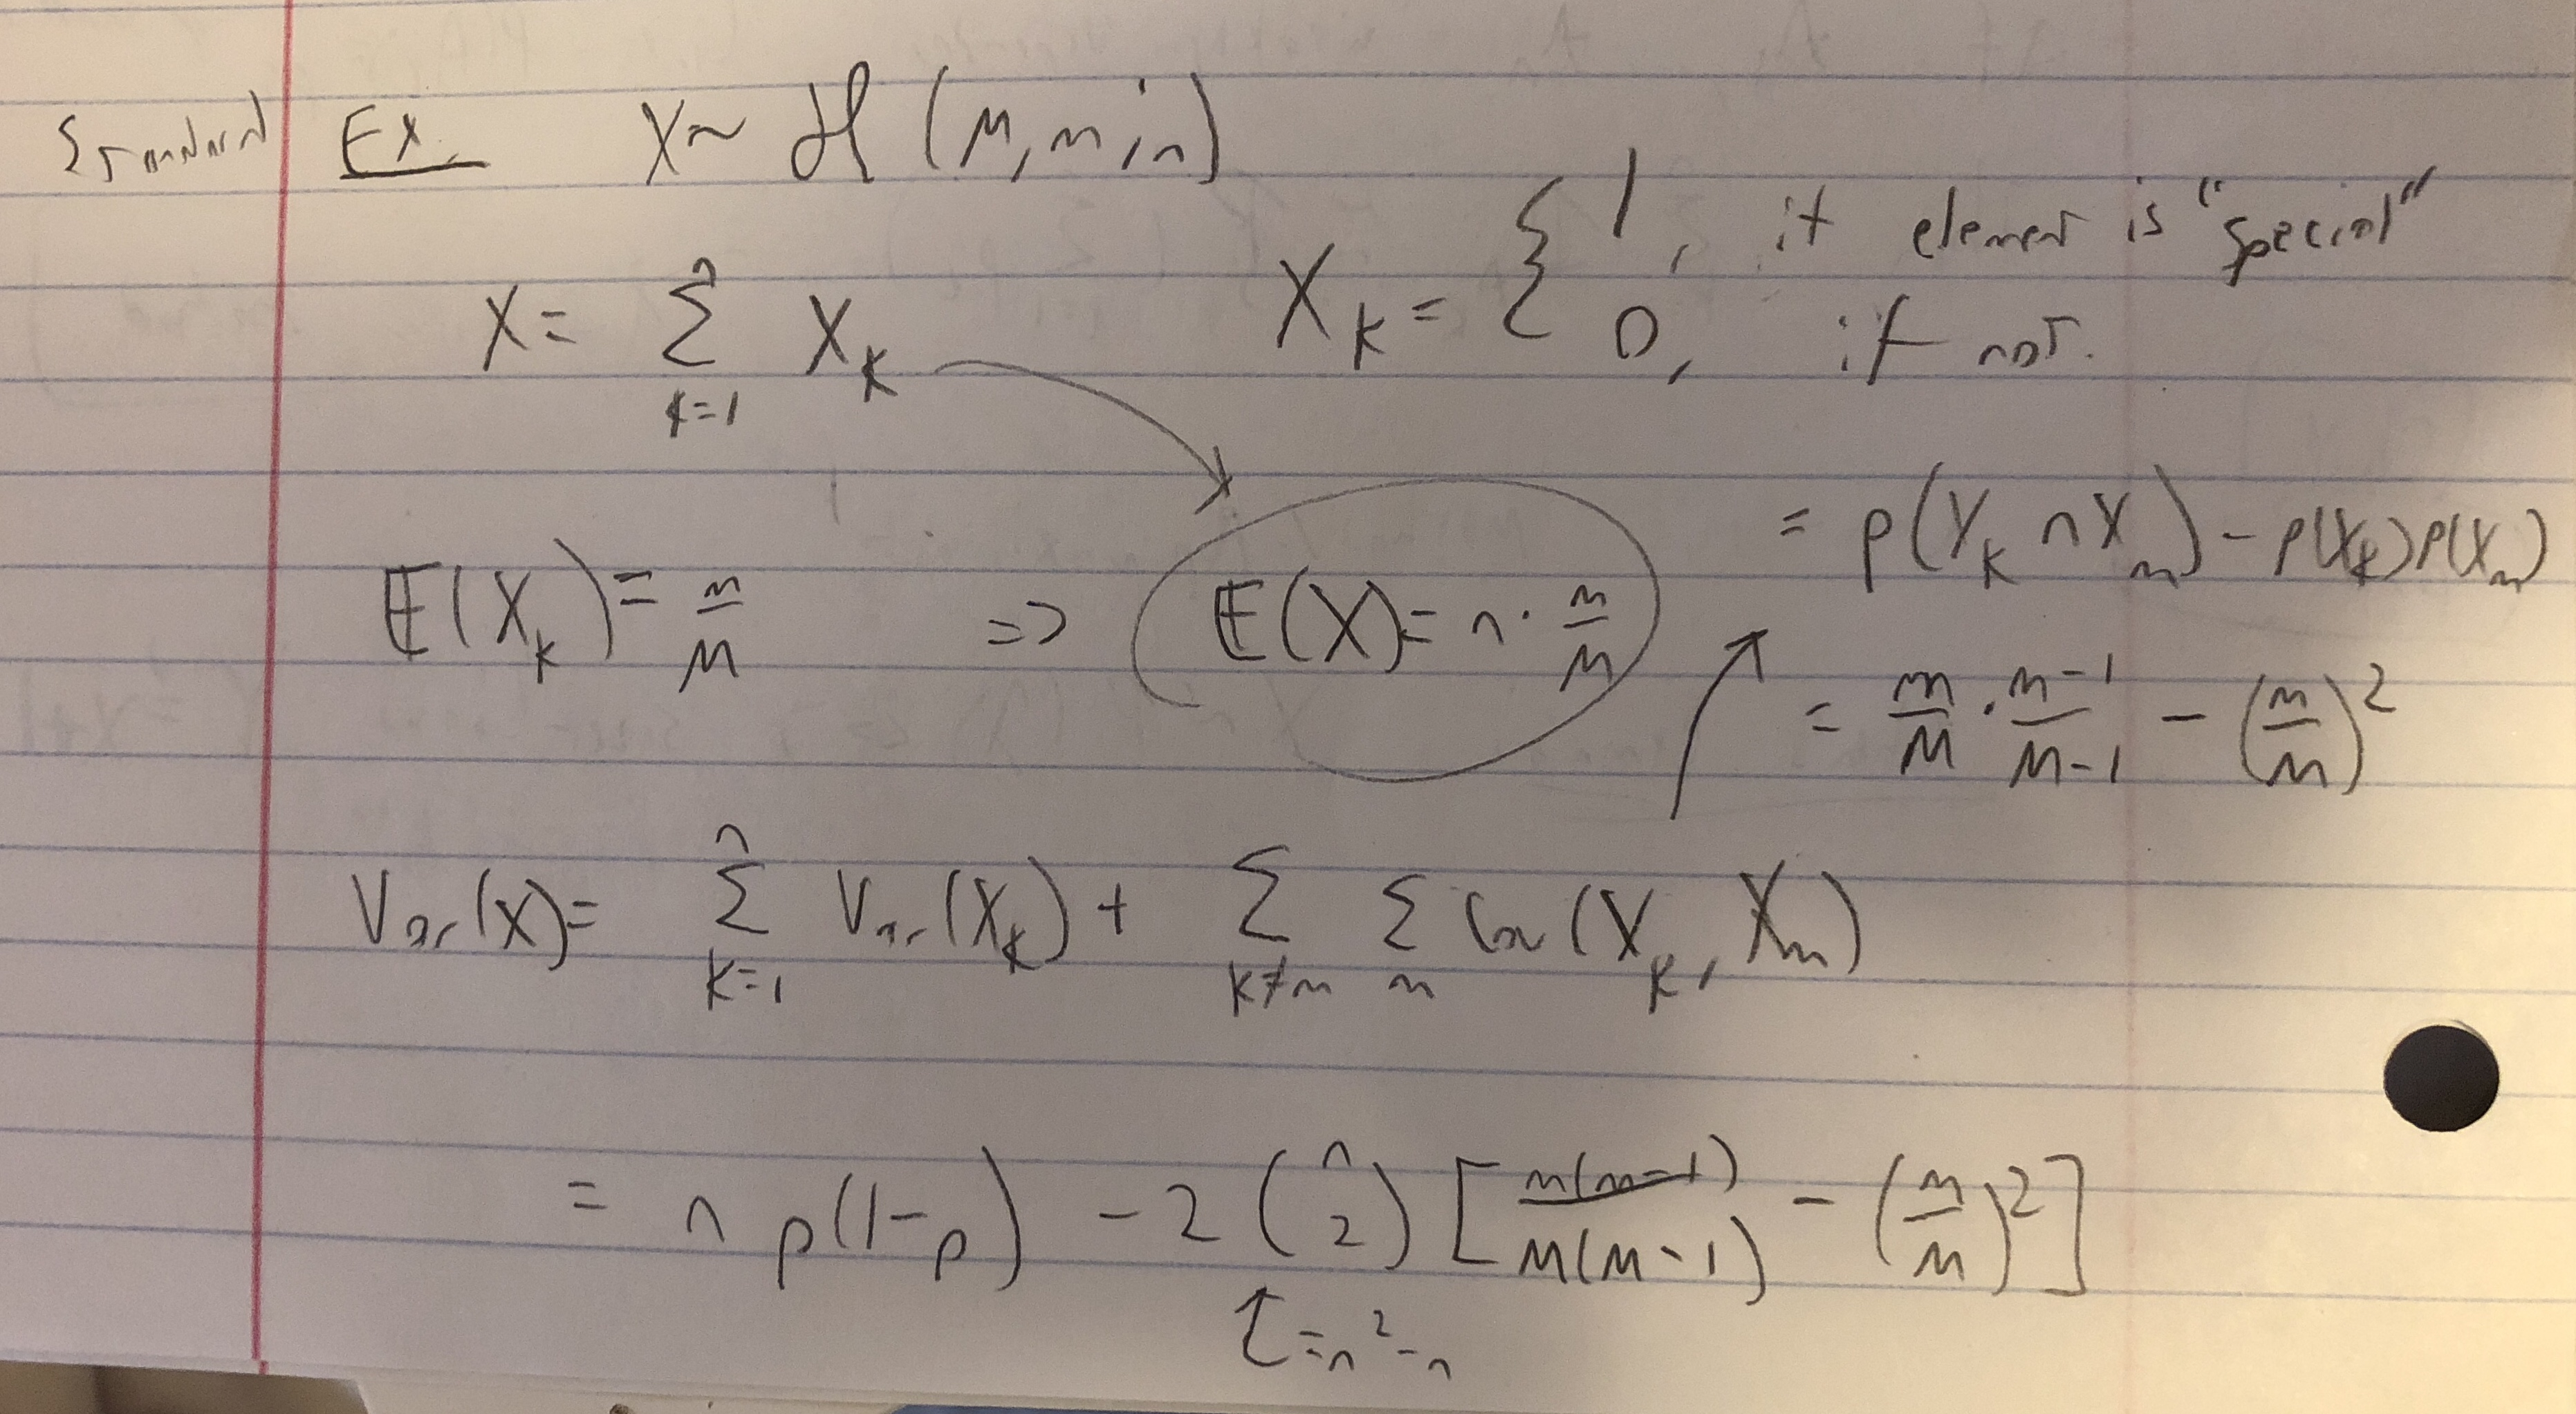
\includegraphics[scale=0.1]{prob_hypergeometric}

\item Variance: \(\Var(X) = \) (find by indicator method)

\end{itemize}


\subsubsection{Indicator Method}

\begin{proposition} If \(\boldsymbol{1}_{A_k}\) is an indicator then

\begin{enumerate}[(a)]

\item

\[
\Cov(\boldsymbol{1}_{A_k}, \boldsymbol{1}_{A_m}) = \E(\boldsymbol{1}_{A_k} \boldsymbol{1}_{A_m}) - \E(\boldsymbol{1}_{A_k}) \E(\boldsymbol{1}_{A_m}) = \Pr(A_k \cap A_m) - \Pr(A_k) \Pr(A_m)
\]

\item

\[
\Var(\boldsymbol{1}_{A_k} ) = \E(\boldsymbol{1}_{A_k} ^2) = \E(\boldsymbol{1}_{A_k} )^2 = \Pr(A_k) - (\Pr(A_k))^2
\]

\end{enumerate}
\end{proposition}

\begin{theorem} \(X\) is independent of \(Y\) if and only if \(X\) is independent of \(\boldsymbol{1}_A\), \(A \in Y\). \end{theorem}

Example problems: 505A Homework 3 problem 9(a)

Worked examples in p. 56 - 59 of Grimmett and Stirzaker 3rd edition.

\subsubsection{Linear transformations of random variables}

\subsubsection{Poisson Paradigm (Poisson approximation for indicator method)}

\begin{theorem} (Theorem 4.12.9, p. 129 of Grimmett and Stirzaker.) Let \(A_i\) be an event. If \(X = \sum_{i=1}^m \boldsymbol{1}_{A_i}\) where \(\boldsymbol{1}_{A_i}\) is an indicator variable for \(A_i\), and the \(A_i\) are only weakly dependent on each other, then 

\[
\text{As } m \to \infty, \ \ X \sim \operatorname{Poisson}(\E(X))
\]

More specifically, let \(B_i\) be \(n\) independent Bernoulli random variables with probabilities \(p_i\). If \(Y = \sum_{i=1}^n B_i\) then 

\[
\text{As } n \to \infty, \ \ Y \sim \operatorname{Poisson} \bigg(\E \bigg(\sum_i B_i \bigg) \bigg) = \operatorname{Poisson}\bigg(\sum_i \E B_i \bigg) = \operatorname{Poisson}\bigg(\sum_i p_i \bigg) 
\]

\end{theorem}

\subsubsection{Asymptotic Distributions}

\begin{proposition}
\[
e^x = \lim_{n \to \infty} \bigg( 1 + \frac{x}{n}\bigg)^n
\]
\end{proposition}

\begin{theorem} \label{prob.stirling} \textbf{Stirling's Formula}: 

\[
n! \approx n^ne^{-n} \sqrt{2\pi n}
\]
\end{theorem}

%%%%%%%% Example Problems That Will Likely Appear on Midterm %%%%%%%%%%%%%
\subsection{Worked problems}

\subsubsection{Example Problems That Will Likely Appear on Midterm}

\textbf{Fall 2011 Problem 1 (same as HW1 problem 5; similar to HW3 problem 2(5); likely to be question 1 on the midterm.)} True or false: if \(A\) and \(B\) are events such that \( 0 < \Pr(A) < 1\) and \(\Pr(B \mid A) = \Pr(B \mid A^c)\), then \(A\) and \(B\) are independent.

\textbf{Solution.} \(A\) and \(B\) are independent if and only if 

\[
\Pr(A \cap B) = \Pr(A)\cdot\Pr(B)
\]

We know that \[ \Pr(B) = \Pr(B|A)\cdot \Pr(A) + \Pr(B|A^c)\cdot\Pr(A^c)  \]

\[
= \Pr(B|A)\cdot \Pr(A) + \Pr(B|A)\cdot (1 - \Pr(A)) = \Pr(B|A)\cdot \Pr(A) + \Pr(B|A) - \Pr(B|A)\cdot \Pr(A) 
\]

\[
= \Pr(B|A)
\]

Also, we know that since \(\Pr(A) \neq 0\),

\[
\Pr(B|A) = \frac{\Pr(A \cap B)}{\Pr(A)} 
\]

Per above \(\Pr(B|A) = \Pr(B)\), so we have

\[
\Pr(B) = \frac{\Pr(A \cap B)}{\Pr(A)} 
\]

\[
\Pr(A \cap B)= \Pr(A) \cdot \Pr(B)
\]

which is what we were trying to prove. So the answer is \(\boxed{\text{true.}}\)

\textbf{Similar problem: HW3 Problem 2(5).} Verify: \(\E(X \mid Y) = \E(X)\) if \(X\) and \(Y\) are independent.

\textbf{Solution.} \(X\) and \(Y\) are independent if and only if

\[
\Pr(X \cap Y) = \Pr(X)\cdot\Pr(Y) \iff \Pr(X = x \cap Y = y) = \Pr(X = x) \Pr(Y = y)
\]

\[
\iff \Pr(X = x \mid Y = y) \cdot \Pr(Y = y) =  \Pr(X = x) \Pr(Y = y) \iff \Pr(X = x \mid Y = y) = \Pr(X = x)
\]

\[
\implies E(X \mid Y) = \sum_x x \cdot \Pr(X = x \mid Y = y ) = \sum_x x \cdot \Pr(X = x ) = \E(X)
\]


\textbf{Fall 2014 Problem 1 (likely to be question 2 on the midterm).} Let \(A\) and \(B\) be two events with \(0 < \Pr(A) < 1, \ 0 < \Pr(B) < 1\). Define the random variables \(\xi = \xi(\omega)\) and \(\eta = \eta(\omega)\) by

\[
\xi(\omega) = \begin{cases} 
      5 & \text{ if } \omega \in A \\
      -7 &  \text{ if } \omega \notin A 
   \end{cases}, \ \ \ \ \eta(\omega) = \begin{cases} 
      2 & \text{ if } \omega \in B \\
      3 &  \text{ if } \omega \notin B 
   \end{cases}
\]

True or false: the events \(A\) and \(B\) are independent if and only if the random variables \(\xi\) and \(\eta\) are uncorrelated?

\textbf{Solution.} (\(\implies\)) Suppose \(A\) and \(B\) are independent. Then \(\xi\) and \(\eta\) are uncorrelated if and only if \(\E(\xi \eta ) = \E(\xi) \E(\eta)\). We can write \(\xi = 5 \cdot \boldsymbol{1}_A - 7 \cdot \boldsymbol{1}_{A^c}\) and \(\eta = 2 \cdot \boldsymbol{1}_B + 3 \cdot \boldsymbol{1}_{B^c}\). So we have

\[
\xi \eta = (5 \cdot \boldsymbol{1}_A - 7 \cdot \boldsymbol{1}_{A^c})(2 \cdot \boldsymbol{1}_B + 3 \cdot \boldsymbol{1}_{B^c}) = 10 \cdot \boldsymbol{1}_{A \cap B} +15 \cdot \boldsymbol{1}_{A \cap B^c} - 14 \cdot \boldsymbol{1}_{A^c \cap B} - 21 \cdot \boldsymbol{1}_{A^c \cap B^c}
\]

\[
\implies \E(\xi \eta ) = 10 \Pr(A \cap B) +15\Pr(A \cap B^c) - 14 \Pr(A^c \cap B) - 21\Pr(A^c \cap B^c)
\]

Then

\[
\E(\xi) \E(\eta) = (5 \Pr(A) - 7 \Pr(A^c))(2 \Pr(B) + 3 \Pr(B^c)) 
\]

\[
= 10\Pr(A \cap B) + 15 \Pr(A \cap B^c) - 14 \Pr(A^c \cap B) - 21 \Pr(A^c \cap B^c) = \E(\xi \eta )
\]

where the second-to-last step follows from the independence of \(A\) and \(B\). Therefore \(\eta\) and \(\xi\) are uncorrelated.

(\(\impliedby\)) Now suppose \(\eta\) and \(\xi\) are uncorrelated. Then \(\xi\) and \(\eta\) are independent if and only if \(\Pr(\xi \cap \eta) = \Pr(\xi) \Pr(\eta)\). Define

\[
\alpha(\omega) =  \xi(\omega) + 7 = \begin{cases} 
      12 & \text{ if } \omega \in A \\
      0 &  \text{ if } \omega \notin A 
   \end{cases}, \ \ \ \ \beta(\omega) =  \eta(\omega) - 3 = \begin{cases} 
      -1 & \text{ if } \omega \in B \\
      0 &  \text{ if } \omega \notin B 
   \end{cases}
\]

Then we have

\[
(\alpha \beta)(\omega) = \begin{cases} 
      -12 & \text{ if } \omega \in A \cap B \\
      0 &  \text{ otherwise} 
   \end{cases}
\]

Then

\[
\E(\xi \eta) = \E\big[ (\alpha - 7)(\beta + 3)\big] = \E(\alpha \beta) + 3 \E(\alpha) - 7 \E(\beta) - 21
\]

\[
\E(\xi) \E(\eta) = (\E(\alpha) - 7) (\E(\beta) + 3) = \E(\alpha) \E(\beta) - 7 \E(\beta) + 3 \E(\alpha) - 21
\]

Since by assumption \( \E(\xi \eta)  = \E(\xi) \E(\eta) \), this yields \(\E(\alpha \beta) = \E(\alpha) \E(\beta) \). But

\[
\E(\alpha \beta) = -12 \Pr(A \cap B), \ \ \ \ \ \E(\alpha) \E(\beta) = 12 \Pr(A) (-1) \Pr(B) = -12\Pr(A)\Pr(B)
\]

Therefore \(\Pr(\xi \cap \eta) = \Pr(\xi) \Pr(\eta)\) and \(\xi\) and \(\eta\) are independent.

%\textbf{Fall 2009 Problem 4 (Very similar).} Let \(X\) and \(Y\) be two random variables, both taking only two values. Show that if they are uncorrelated, then they are independent.
%
%\textbf{Solution.} Let \(X\) and \(Y\) have the following pmfs: \(\Pr(X = a) = p, \Pr(X = b) = 1-p; \ \ \ \Pr(Y = c) = q, \Pr(Y = d) = 1  -q \). Suppose \(X\) and \(Y\) are uncorrelated; that is, \(\E(XY) = \E(X)\E(Y)\). Then \(X\) and \(Y\) are independent if \(\Pr(X \cap Y) = \Pr(X) \Pr(Y)\). Since these random variables take on only two values each, this can also be expressed as \( \Pr(X = a \cap Y = c) = \Pr(X = a) \Pr(Y = c)\). 
%
%Begin by defining new variables \(\alpha = X - b\) and \(\beta = Y - d\). Then we have
%
%\[
%\E(\alpha \beta) = \E( (X - b)(Y - d)) = \E(XY) - b \E(Y) -d \E(X) + bd
%\]
%
%\[
%\E(\alpha) \E(\beta) = \E(X-b) \E(Y - d) = \E(X)\E(Y) -b \E(Y) -d \E(X) + bd
%\]
%
%Since by assumption \(\E(XY) = \E(X)\E(Y)\), this yields \(\E(\alpha \beta)  = \E(\alpha) \E(\beta) \). But \(\E(\alpha) = p(a-b) = (a - b) \Pr(X = a)\), \(\E(\beta) = q(c-d) = (c -d) \Pr(Y = c)\), \(\E(\alpha \beta) = (a-b)(c-d)pq = (a - b)(c - d) \Pr(X = a \cap Y = c)\). Therefore
%
%\[
%\E(\alpha \beta)  = \E(\alpha) \E(\beta)  \iff  (a - b)(c - d) \Pr(X = a \cap Y = c) = (a - b) \Pr(X = a) (c -d) \Pr(Y = c)
%\]
%
%\[
%\iff \Pr(X = a \cap Y = c) = \Pr(X = a)  \Pr(Y = c)
%\]
%
%which proves the independence of \(X\) and \(Y\).

\textbf{HW1 Problem 8.} Two people, \(A\) and \(B\), are involved in a duel. The rules are simple: shoot at each other once; if at least one is hit, the duel is over, if both miss, repeat (go to the next round), and so on. Denote by \(p_A\) and \(p_B\) the probabilities that \(A\) hits \(B\) and \(B\) hits \(A\) with one shot, and assume that that hitting/missing is independent from round to round. Compute the probabilities of the following events: (a) the duel ends and \(A\) is not hit; (b) the duel ends and both are hit; (c) the duel ends after round number \(n\); (d) the duel ends after round number \(n\) GIVEN that \(A\) is not hit; (e) the duel ends after \(n\) rounds GIVEN that both are hit; (f) the duel goes on forever.

\textbf{Solution.} \begin{enumerate}[(a)]

% 8a
\item Let \(A_k\) denote the event that the duel is ended by \(A\) shooting \(B\) in the \(k\)th round (with neither person being shot in the first \(k - 1\) rounds). Note that \( \{A_k | k = 1, 2, \ldots\}\) are all mutually exclusive. Therefore the probability of the duel ending without \(A\) being hit is \(\sum_{k=1}^\infty A_k\). Because the probabilities in each round are constant and independent, 

\[
A_k = (1 - p_A)^{{k-1}}p_A(1 - p_B)^{k}
\]

So the probability that the duel ends and \(A\) is not hit is

\[
\sum_{k=1}^\infty A_k = \sum_{k=1}^\infty (1 - p_A)^{{k-1}}p_A(1 - p_B)^{k} = p_A (1 - p_B)\sum_{k=1}^\infty (1 - p_A)^{{k-1}}(1 - p_B)^{k-1} 
\]

This is an infinite geometric series. Since the ratio \((1 - p_A)(1 - p_B)\) has absolute value less than 1, the sum can be calculated.

\[
\sum_{k=1}^\infty A_k = p_A (1 - p_B) \cdot \frac{1}{1 - (1 - p_A)(1 - p_B)} = \frac{p_A (1 - p_B) }{p_A + p_B - p_Ap_B} = \boxed{\frac{p_A (1 - p_B) }{p_A(1 - p_B) + p_B}}
\]

% 8b
\item Similar to part (a). Let \(C_k\) denote the event that the duel is ended with both players being shot in the \(k\)th round (with neither person being shot in the first \(k - 1\) rounds). Again, \( \{C_k | k = 1, 2, \ldots\}\) are all mutually exclusive, so the probability of the duel ending in these circumstances is \(\sum_{k=1}^\infty C_k\). We have

\[
C_k = (1 - p_A)^{{k-1}}p_A(1 - p_B)^{k-1}p_B
\]

\[
\sum_{k=1}^\infty C_k = \sum_{k=1}^\infty (1 - p_A)^{{k-1}}p_A(1 - p_B)^{k-1}p_B = p_A p_B\sum_{k=1}^\infty (1 - p_A)^{{k-1}}(1 - p_B)^{k-1} 
\]

\[
= p_A p_B \cdot \frac{1}{1 - (1 - p_A)(1 - p_B)} = \boxed{ \frac{p_A p_B }{p_A + p_B - p_Ap_B} }
\]

Note that this value is less than the answer from part (a) if \(p_B < \frac{1}{2}\) and greater if \(p_B > \frac{1}{2}\)

% 8c
\item Let \(B_k\) denote the event that the duel is ended by \(B\) shooting \(A\) in the \(k\)th round (with neither person being shot in the first \(k - 1\) rounds), with

\[
B_k = (1 - p_A)^{{k}}p_B(1 - p_B)^{k-1}
\]

Let \(A_k\) and \(C_k\) be defined as above. Note that \(\{A_k | k = 1, 2, \ldots\} , \{B_k | k = 1, 2, \ldots\}, \{C_k | k = 1, 2, \ldots\}\) are all mutually exclusive, and that the event that the duel ends in round \(n\) is \(\{A_n \cup B_n \cup C_n\}\). So the probability of the duel ending in round \(n\) is

\[
\Pr(A_n \cup B_n \cup C_n) = \Pr(A_n) + \Pr(B_n) + \Pr(C_n) 
\]

\[
= (1 - p_A)^{n-1}p_A(1 - p_B)^{n} + (1 - p_A)^{{n}}p_B(1 - p_B)^{n-1} + (1 - p_A)^{{n-1}}p_A(1 - p_B)^{n-1}p_B
\]

\[
= (1 - p_A)^{n-1}(1 - p_B)^{n-1} \big[p_A(1 - p_B) + (1 - p_A)p_B + p_Ap_B \big]
\]

\[
= \boxed{(1 - p_A)^{n-1}(1 - p_B)^{n-1} (p_A + p_B - p_Ap_B )}
\]

% 8d
\item Let \(A_k\), \(B_k\), \(C_k\) be defined as above. The event that the duel ends at round \(n\) without \(A\) being hit is given by \(\{ A_n\} \). 

\[
\Pr(A_n) = \boxed{(1 - p_A)^{{n-1}}p_A(1 - p_B)^{n}}
\]

% 8e
\item Let \(A_k\), \(B_k\), \(C_k\) be defined as above. The event that the duel ends at round \(n\) with both players being hit is given by \(\{ C_n\} \). 

\[
\Pr(C_n) = \boxed{(1 - p_A)^{{n-1}}p_A(1 - p_B)^{n-1}p_B}
\]

% 8e
\item Let \(A_k\), \(B_k\), \(C_k\) be defined as above. The probability that the duel never ends is equal to 1 - the probability that the duel ends at some point, which is  \(\{A_k | k = 1, 2, \ldots\} \cup \{B_k | k = 1, 2, \ldots\} \cup \{C_k | k = 1, 2, \ldots\}\). Since all of these events are mutually exclusive, we have

\[
1 - \Pr(\{A_k | k = 1, 2, \ldots\} \cup \{B_k | k = 1, 2, \ldots\} \cup \{C_k | k = 1, 2, \ldots\}) = 1 - \sum_{k = 1}^\infty \big(A_k + B_k + C_k\big)
\]

\[
= 1 - \sum_{k=1}^\infty \big( (1 - p_A)^{{k-1}}p_A(1 - p_B)^{k} + (1 - p_A)^{{k}}p_B(1 - p_B)^{k-1} + (1 - p_A)^{{k-1}}p_A(1 - p_B)^{k-1}p_B \big)
\]

\[
= 1 -   \big[p_A(1 - p_B) + (1 - p_A)p_B + p_Ap_B \big] \sum_{k=1}^\infty (1 - p_A)^{k-1}(1 - p_B)^{k-1} 
\]

\[
=  1 -  \big[ p_A1 - p_A p_B) + p_B - p_A)p_B + p_Ap_B \big] \cdot \frac{1}{1 - (1 - p_A)(1 - p_B)}
\]

\[
=1 -  \frac{p_A - p_Ap_B + p_B - p_Ap_B + p_Ap_B}{p_A + p_B - p_Ap_B} = 1 -  \frac{p_A + p_B - p_Ap_B}{p_A + p_B - p_Ap_B} = \boxed{0}
\]

\end{enumerate}

%\textbf{Independence Problem 09/24 (number 2 on some qual, likely to be problem 3 on the test)} 
%
%\textbf{Solution.} \(X\) is independent of \(Y\) if and only if \(X\) is independent of \(\boldsymbol{1}_A\), \(A \in Y\). 
%
%\[
%\implies \E(X \mid Y) = \E(X)
%\]
%
%\[
%\E( \E(X \mid Y) \boldsymbol{1}_A) = \E(X \boldsymbol{1}_A) = \E(X) \E(\boldsymbol{1}_A)
%\]
%
%where the last step follows by independence.

\textbf{Similar: HW3 Problem 2 (parts 1 - 4).} Verify:

\begin{enumerate}[(1)]

\item \(\E(\E(X\mid Y)) = \E(X)\)

\item \( \E(g(Y) X \mid Y) = g(Y) \E(X \mid Y) \)

\item \(\Cov ( \E(X \mid Y), Y ) = \Cov(X , Y)\)

\item \(Y\) and \(X - \E(X \mid Y)\) are uncorrelated.

\end{enumerate}

\textbf{Solution.} \begin{enumerate}[(1)]

%1
\item 

\[
\E\big(\E(X\mid Y)\big) = \sum_y \E(X \mid Y) \Pr(Y = y) = \sum_y \bigg[ \sum_x x \cdot \Pr(X = x \mid Y = y) \Pr(Y = y) \bigg]
\]

\[
= \sum_y \bigg[ \sum_x x \cdot \Pr(X = x \cap Y = y) \bigg] = \sum_y \bigg[ \sum_x x \cdot \Pr(Y= y \mid X = x) \cdot \Pr(X = x) \bigg]
\]

\[
= \sum_x \bigg[ x \cdot \Pr(X = x) \cdot \sum_y \big( \Pr(Y= y \mid X = x) \big) \bigg] = \sum_x \bigg[ x \cdot \Pr(X = x) \cdot 1 \bigg]
\]

\[
= \E(X)
\]

%%2
\item 2
%
%%\textbf{double check?}
%
%\[
%\E(g(Y)X \mid Y) = \sum_{y} \sum_x g(y) \cdot x \cdot \Pr(g(Y) = g(y) \cap X = x \mid Y = y) 
%\]
%
%\[
%= \sum_{y} \sum_x g(y) \cdot x \cdot \Pr( X = x \mid Y = y) = \sum_{y}  g(y) \sum_x x \cdot \Pr( X = x \mid Y = y) 
%\]
%
%\[
%= \sum_{y}  g(y) \E(X \mid Y = y)
%\]
%
%
%\[
%= g(Y) \E(X \mid Y)
%\]

%3
\item 

\[
\Cov(\E(X \mid Y) , Y) = \E \bigg( \bigg[\E(X \mid Y) - \E \big(\E(X \mid Y) \big) \bigg] \bigg[Y - \E(Y) \bigg] \bigg)
\]

\[
= \E \bigg( \bigg[\E(X \mid Y) - \E (X) \bigg] \bigg[Y - \E(Y) \bigg] \bigg) = \E \bigg( \E(X \mid Y)Y  - \E (X) Y -  \E(X \mid Y)\E(Y) +  \E(X)\E(Y)  \bigg)
\]

\[
= \E \big( \E(X \mid Y)Y\big)  -  \E (X) \E( Y)  - \E(Y) \E \big( \E(X \mid Y) \big) +   \E(X)\E(Y) = \E \big( \E(X \mid Y)Y\big)  - \E(Y) \E(X)
\]

\[
= \E(XY) - \E(X) \E(Y) = \Cov(X, Y)
\]

%4
\item \(Y\) and \(X  - \E(X \mid Y)\) are uncorrelated if and only if \( \Cov \big(Y, X - \E(X \mid Y) \big) = 0 \iff \E(Y \cdot \big[ X - \E(X \mid Y)\big] ) - \E(Y) \E( X - \E(X \mid Y)) = 0 \).

\[
\E(Y \cdot \big[ X - \E(X \mid Y)\big] ) -  \E(Y) \E( X - \E(X \mid Y))= \E(Y X - Y \E(X \mid Y) ) -  \E(Y) \E( X) +  \E(Y) \E \big( \E(X \mid Y)) \big)
\]

\[
= \E(Y X) - \E\big( Y \E(X \mid Y) \big) -  \E(Y) \E( X)  + \E(Y) \E(X) = \E(YX) - \E(YX) = 0
\]

\end{enumerate}

\textbf{Remaining problems are likely to be indicator method.}

%%%%%%%%%%% Problems we did in class that professor mentioned %%%%%%%%%%%%


\subsubsection{Problems we did in class that professor mentioned}

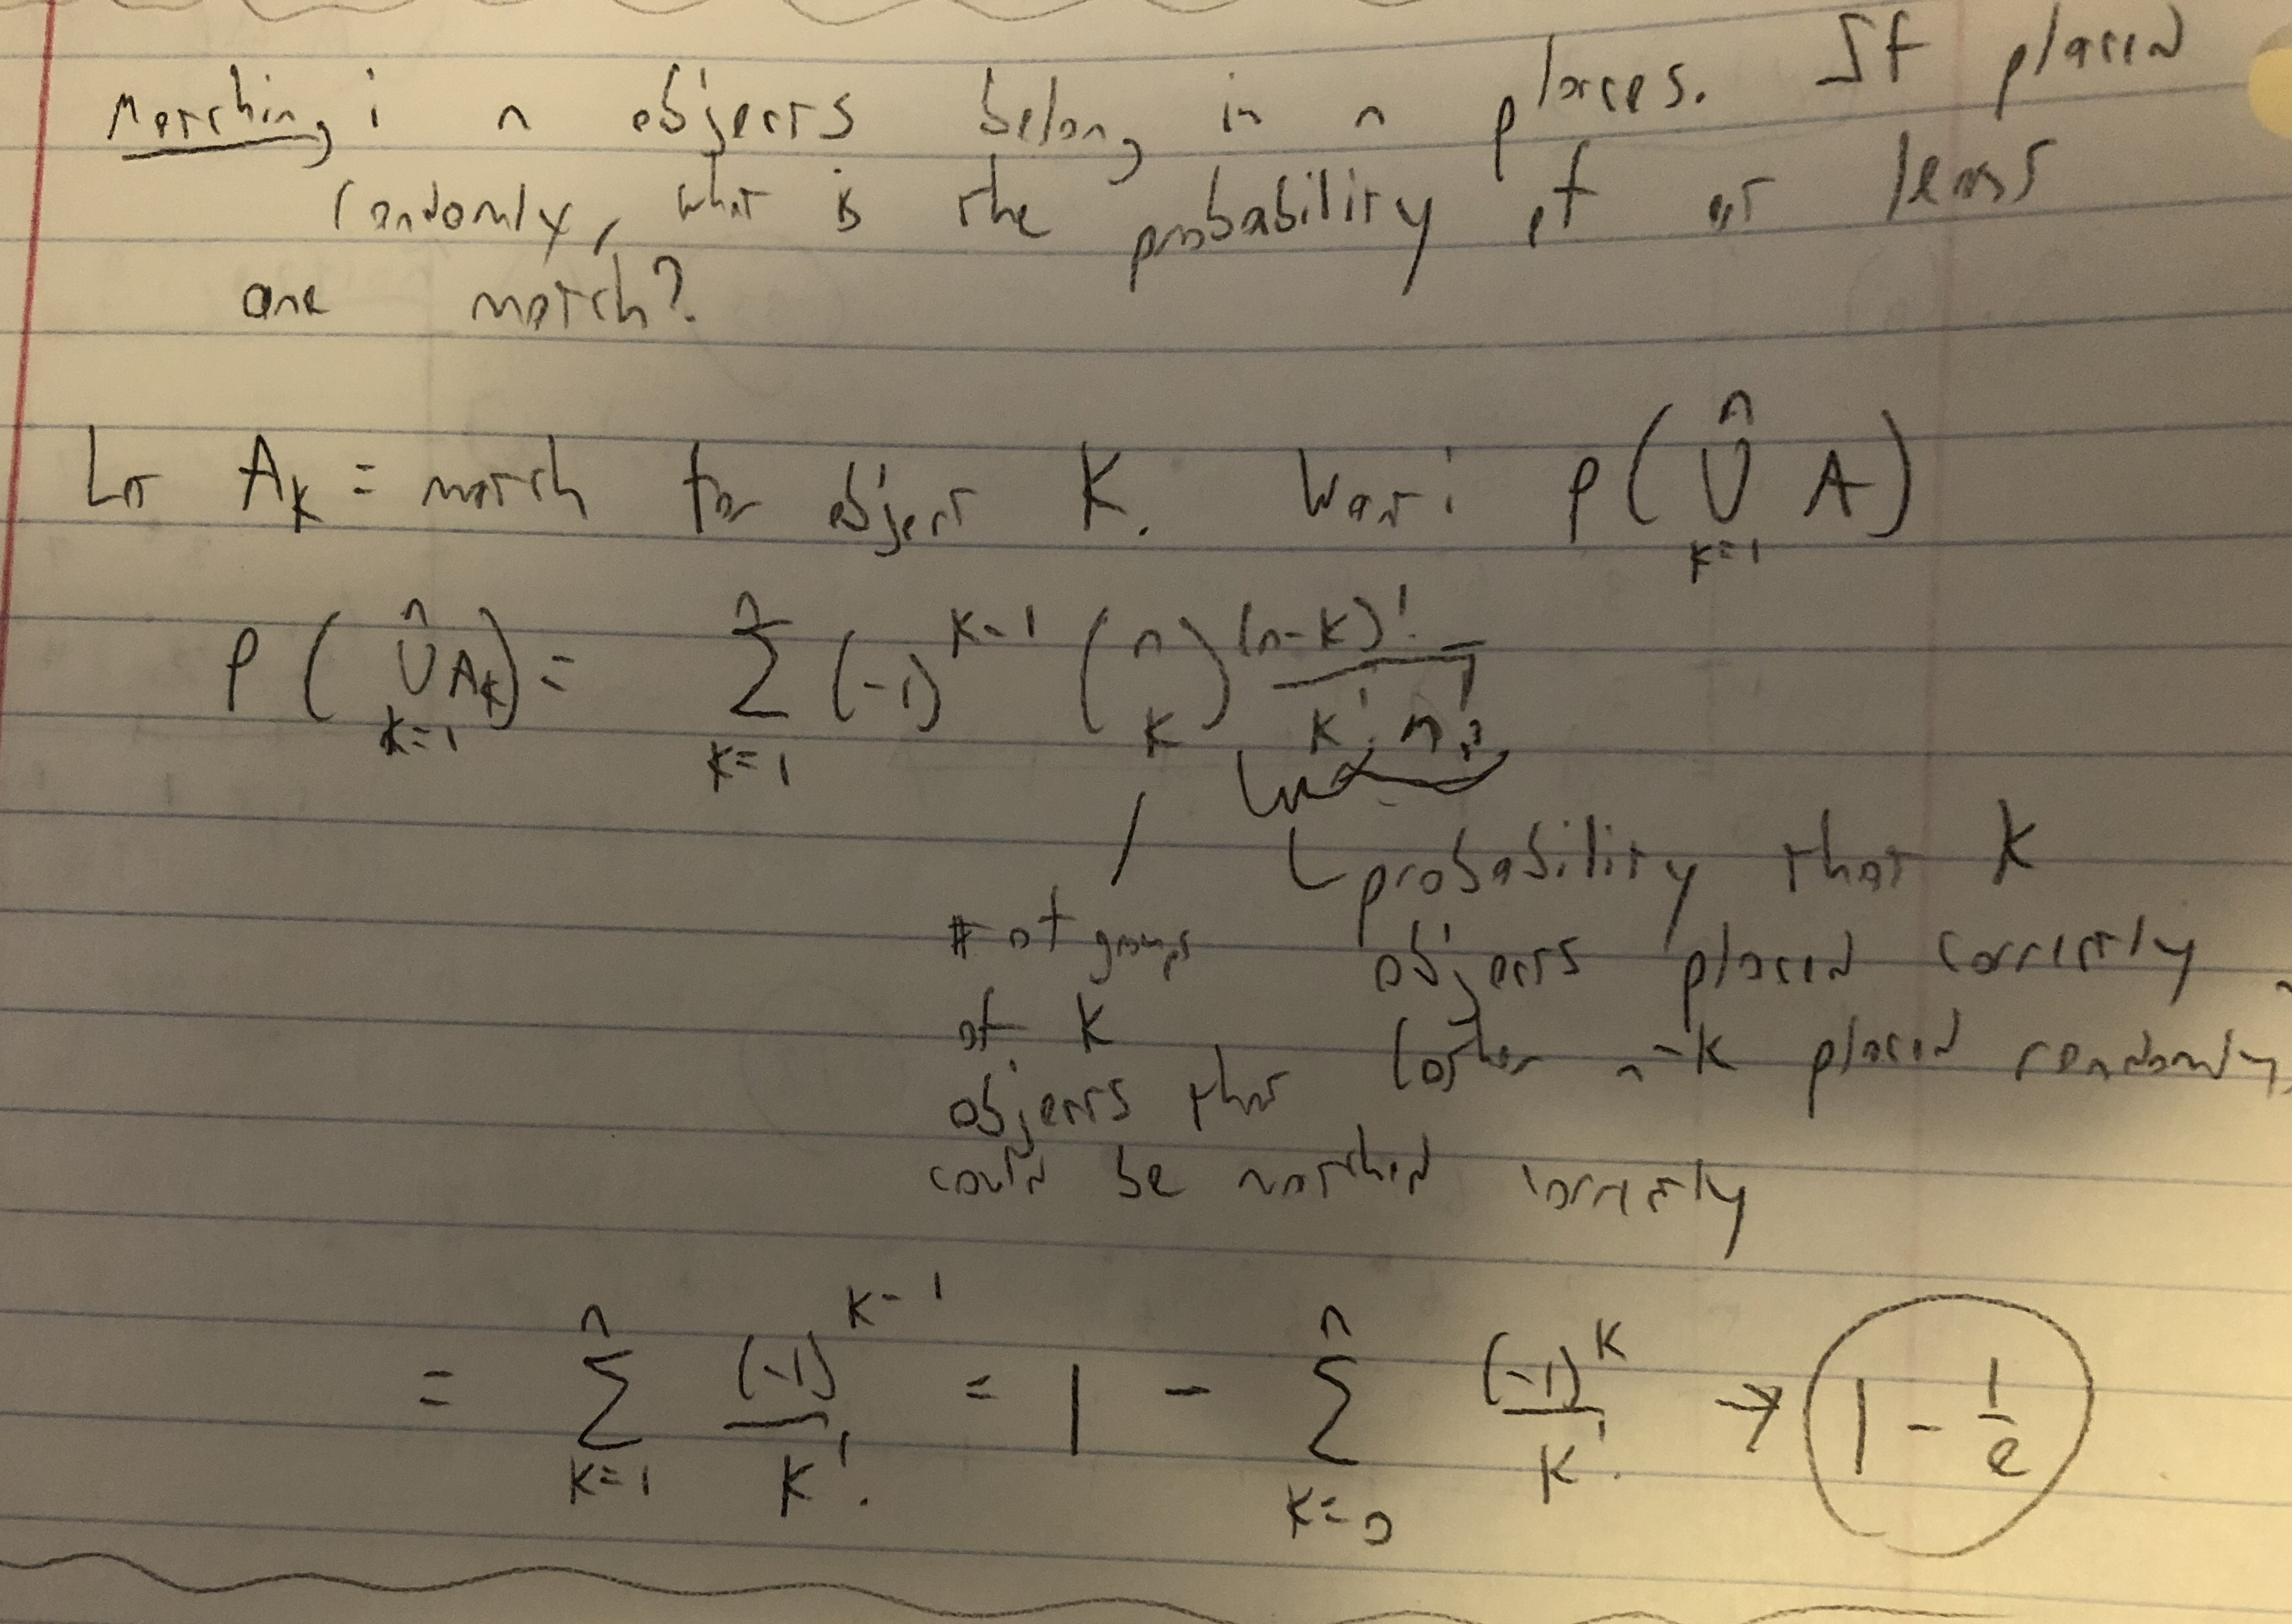
\includegraphics[scale=0.1]{prob_classex_matching}

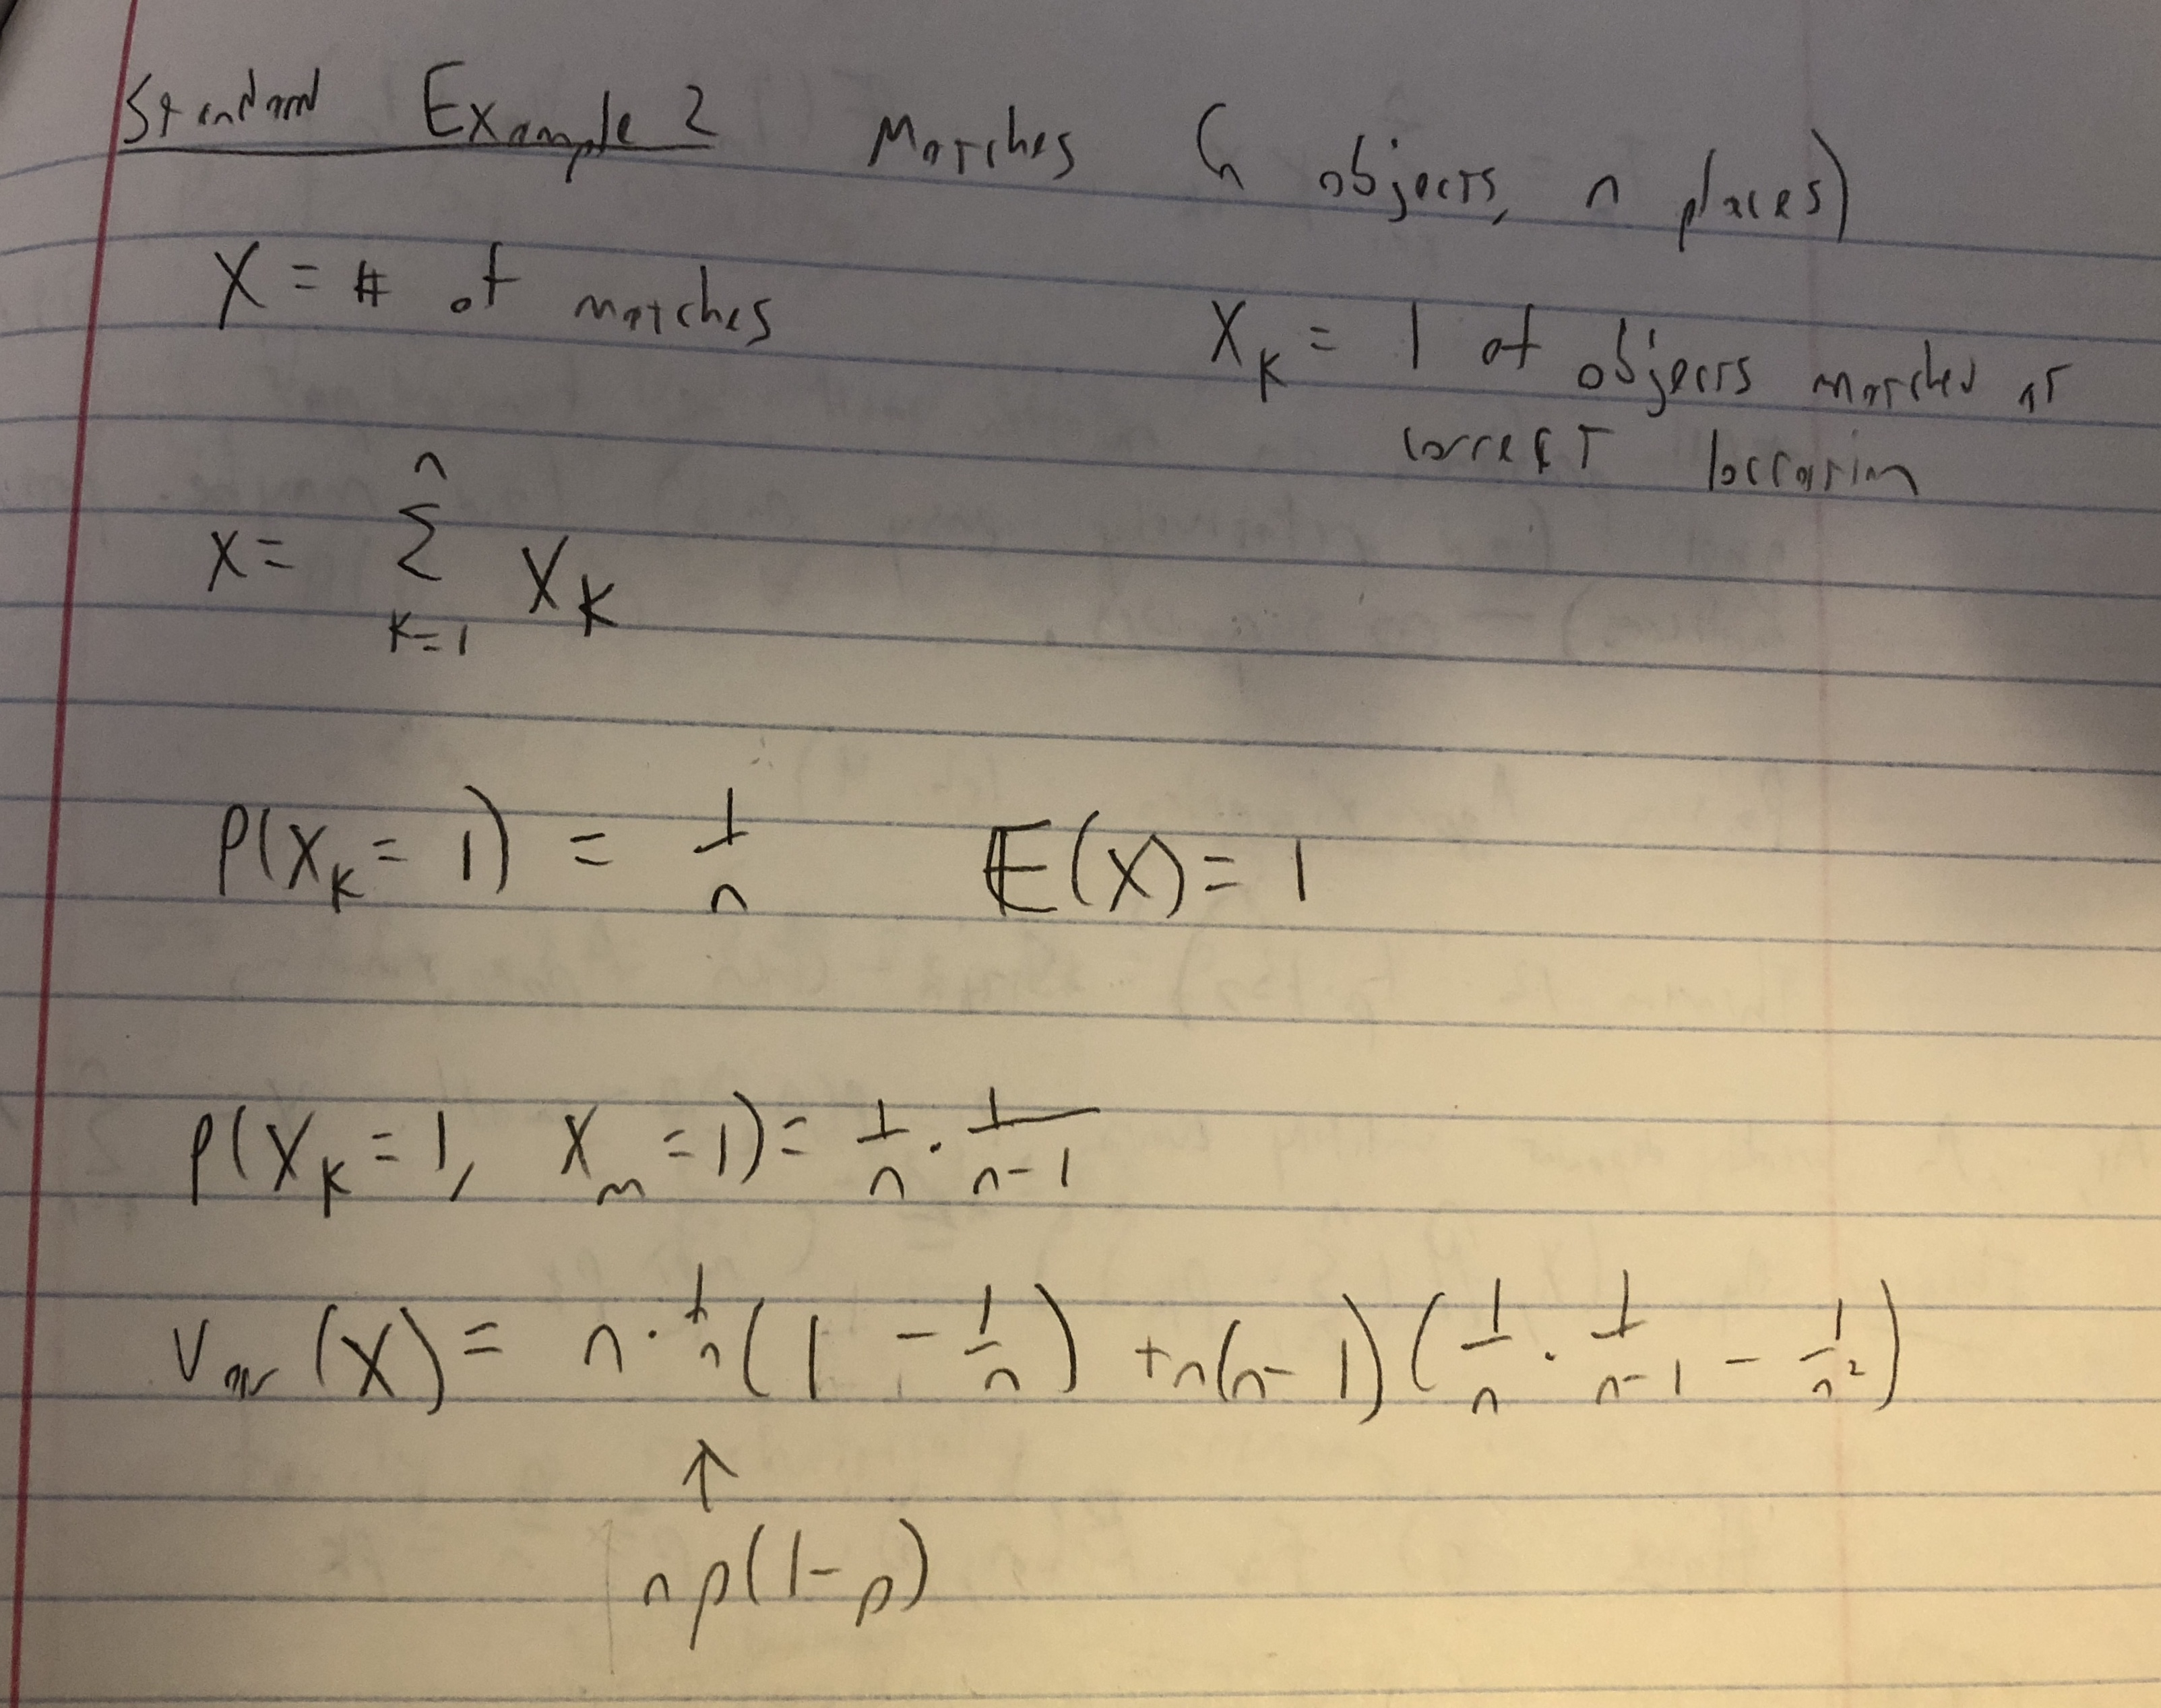
\includegraphics[scale=0.1]{prob_classex_matching2}

\textbf{Variance Problem 09/21}  If \(\E(X \mid Y) = Y, \E(Y \mid X) = X, \E(X^2) < \infty, \E(Y^2) < \infty\), show \(\E(X-Y)^2 = 0 \) (or equivalently, show \(\Pr(X = Y) = 1\)).

\textbf{Solution.} 

\[
\E(X-Y)^2 = \E(X^2 - 2XY + Y^2) = \E(X^2) - 2 \E(XY) + \E(Y^2)
\]

\[
\E(XY) = \E( \E(XY\mid Y)) = \E(Y\E(X\mid Y)) = \E(Y \cdot Y) = \E(Y^2)
\]

Also,

\[
\E(XY) = \E((XY \mid X)) = \E(X \E(Y \mid X)) = \E( X \cdot X) = \E(X^2)
\]

Therefore

\[
\E(X-Y)^2 =0
\]


\textbf{Spring 2018 Problem 2 (did not complete)}

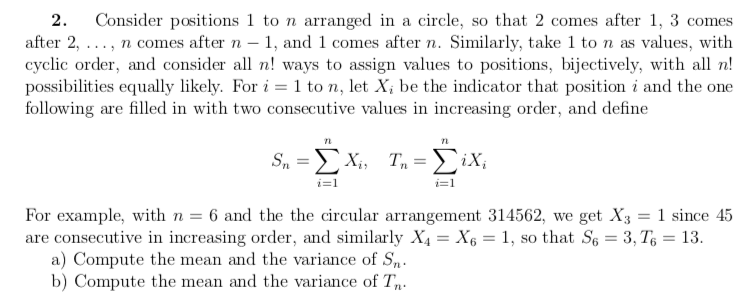
\includegraphics[scale=0.6]{prob_sp18p2}

\textbf{Fall 2008 Problem 2 (HW1 Problem 10).} Consider a lottery with \(n^2\), tickets, of which only \(n\) tickets win prizes. Let \(p_n\) be the probability that, out of \(n\) randomly selected tickets, at least one wins a prize. Compute \(\lim_{n \to \infty} p_n\).

\textbf{Solution.} There are \(\binom{n^2}{n}\) possible sets of \(n\) tickets. The number of these sets that do not contain at least one winner (that is, they only contain members of the \(n^2 - n\) losing tickets) is \(\binom{n^2 - n}{n}\). Therefore the probability of selecting a set of \(n\) tickets that contains at least one winner is

\[
p_n = 1 - \binom{n^2 - n}{n} \bigg/ \binom{n^2}{n} = 1 - \frac{(n^2 - n)!}{n!(n^2 - n - n)!} \bigg/ \frac{(n^2)!}{(n^2 - n)!n!} = 1 - \frac{(n^2 - n)!}{n!(n^2 - 2n)!} \cdot \frac{(n^2 - n)!n!}{(n^2)!}
\]

\[
 = 1 - \frac{(n^2 - n)!}{(n^2 - 2n)!} \cdot \frac{(n^2 - n)!}{(n^2)!} = 1 - \prod_{i=0}^{n-1}(n^2 - n - i)  \bigg/ \prod_{i=0}^{n-1}(n^2 - i) = 1 - \prod_{i=0}^{n-1} \frac{n^2 - n - i}{n^2 - i}
\]

\[
= 1 - \prod_{i=0}^{n-1}\bigg( \frac{n^2 - i}{n^2 - i} -\frac{n}{n^2 - i} \bigg) = 1 - \prod_{i=0}^{n-1}\bigg(1-\frac{n}{n^2 - i} \bigg)
\]

Therefore

\[
\lim_{n \to \infty} p_n = \lim_{n \to \infty} \bigg[ 1 - \prod_{i=0}^{n-1}\bigg(1-\frac{n}{n^2 - i} \bigg) \bigg] = 1 - \lim_{n \to \infty} \prod_{i=0}^{n}\bigg(1-\frac{n}{n^2 - i} \bigg) = 1 - \lim_{n \to \infty} \prod_{i=0}^{n}\bigg(1-\frac{n \cdot \frac{1}{n}}{\frac{n^2}{n} - \frac{i}{n}} \bigg)
\]

\[
= 1 - \lim_{n \to \infty} \prod_{i=0}^{n}\bigg(1-\frac{1}{n - \frac{i}{n}} \bigg) = 1 - \lim_{n \to \infty} \prod_{i=0}^{n}\bigg(1-\frac{1}{n} \bigg) = 1 - \lim_{n \to \infty}  \bigg(1 - \frac{1}{n} \bigg)^n = \boxed{1 - \exp(-1)}
\]

%%%%%%%%%%% Problems we did on homework %%%%%%%%%%%%%%%%%%%%%

\subsubsection{Problems we did on homework}

%\textbf{Fall 2017 Problem 2/Fall 2009 Problem 1 (HW3 Problem 6---most of solution)}
%
%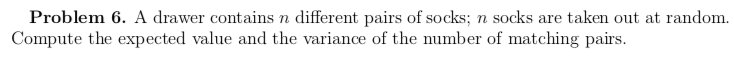
\includegraphics[scale=0.6]{prob_hw3p6}
%
%%\textbf{From Fall 2017 qual, no solutions to quals that late. Not in solutions to past homeworks online. Seems kind of standard, like I might be able to google.}
%
%\textbf{Solution.} Let \(X\) represent the number of matching pairs. At most \(n/2\) pairs can be formed. We have
%
%\[
%\Pr(X = 0) = \frac{\binom{n}{n}2^n }{\binom{2n}{n}} 
%\]
%
%because there are \(\binom{n}{n}\) ways to choose which \(n\) pairs will fail to match, \(2^n\) ways to pick which sock will be chosen in each of these pairs, and \(\binom{2n}{n}\) total ways to pick out \(n\) socks. Next,
%
%\[
%\Pr(X = 1) = \frac{\binom{n}{n - 1}2^{n-1} }{\binom{2n}{n}} 
%\]
%
%because there are \(\binom{n}{n - 1}\) ways to choose which \(n - 1\) pairs will fail to match, \(2^{n-1}\) ways to pick which sock will be chosen in each of these pairs, 1 way to choose which socks will be chosen in the matched pairs, and \(\binom{2n}{n}\) total ways to pick out \(n\) socks. In general,
%
%\[
%\Pr(X = k) = \frac{\binom{n}{n - k}2^{n-k} }{\binom{2n}{n}}  = \frac{(n!)^3 }{(n-k)!k!(2n)!} \cdot 2^{n-k} , \ \ k = 0, 1, \ldots, n/2
%\]
%
%Therefore
%
%\[
%\E(X) = \sum_{k=0}^{n/2} k \cdot  \frac{(n!)^3 }{(n-k)!k!(2n)!} \cdot 2^{n-k} = \boxed{ \frac{(n!)^2}{(2n)!} \sum_{k=1}^{n/2}k \cdot  \binom{n}{k} 2^{n-k} }
%\]
%
%\[
%\Var(X) = \sum_{k=0}^{n/2} k^2 \cdot  \frac{(n!)^3 }{(n-k)!k!(2n)!} \cdot 2^{n-k}  - \bigg(  \frac{(n!)^2}{(2n)!} \sum_{k=1}^{n/2}k \cdot  \binom{n}{k} 2^{n-k} \bigg)^2
%\]
%
%\[
%= \boxed{ \frac{(n!)^2}{(2n)!} \sum_{k=1}^{n/2}k^2 \cdot  \binom{n}{k} 2^{n-k}  - \bigg(  \frac{(n!)^2}{(2n)!} \sum_{k=1}^{n/2}k \cdot  \binom{n}{k} 2^{n-k} \bigg)^2 }
%\]


\textbf{Fall 2017 Problem 3 (HW3 Problem 8---almost full solution)}

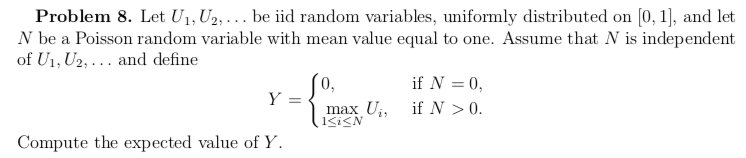
\includegraphics[scale=0.6]{prob_hw3p8}

%\textbf{Some information in notes from 09/24. Also from Fall 2017 qual, no solutions to quals that late. Feel like might be in notes from 100B. Seems kind of standard, might be able to google.}

\textbf{Solution.} 

Since \(Y\) is a function of \(N\), let \(Y = y(N)\). By the Law of the Unconscious Statistician (Theorem \ref{prob.law.of.uncon}),

\[
\E(Y) = \E \big( \E( Y \mid N) \big) = \E \big( \E( \max_{1 \leq i \leq N} U_i \mid N = n ) \big) 
\]

Let \( Z_n = \max_{1 \leq i \leq n} U_i  \). The cdf of \(Z_n\) can be calculated as follows:

\[
\Pr(Z_n \leq x) = \Pr(  \max_{1 \leq i \leq n} U_i  \leq x) = \Pr(U_1 \leq x \cap U_2 \leq x \cap \ldots \cap U_n \leq x) = x^n
\]

for \(x \in [0, 1]\). Therefore the pdf of \(Z_n\) is its derivative, \(nx^{n-1}\). So we have

\[
 \E( \max_{1 \leq i \leq N} U_i \mid N = n ) = \E(Z_n) = \int_{0}^1 x n x^{n-1} dx = n \int_0^1 x^n dx = n \frac{x^{n+1}}{n+1} \bigg|_0^1 = \frac{n}{n+1}
\]

Plugging this into the expression for \(\E(Y)\) yields

\[
\E(Y) = \E \bigg( \frac{N}{N+1} \bigg) = \sum_{n=1}^\infty \frac{n}{n+1} \Pr(N = n) = \sum_{n=1}^\infty \frac{n}{n+1} \frac{\exp(-1)1^n}{n!} = \boxed{ \frac{1}{e} \sum_{n=1}^\infty \frac{n}{(n+1)!}}
\]


%\textbf{Spring 2016 Problem 3 (HW3 Problem 5---currently incomplete)} Fix positive integers \(m \leq n\) with \(n > 4\). Suppose \(m\) people sit at a circular table with \(n\) seats, with all \(n\) arrangements equally likely. A seat is called isolated if it isoccupied and both adjacent seats are vacant. Find the mean and variance of the number of isolated seats.
%
%\textbf{Solution.} There are \(\binom{n}{m}\) possible seatings, although only \( \binom{n-1}{m}\) of these are unique up to rotation. Let \(X\) be the number of isolated seats. Clearly if \(m \in \{0,  n-1, n\}\), there can't be any isolated seats, so in these cases, \(\E(X \mid m \in \{0, n-1, n\}) = 0, \ \Var(X  \mid m \in \{0, n-1, n\}) = 0\). Similarly, if \(m = 1\), there must be one isolated seat, so \(E(X \mid m = 1) = 1, \ \Var(X \mid m = 1) = 0\). 
%
%\
%
%Let \(A_i\) be the event that \(i\) people are seated next to at least one more person. If \(m = 2\), \(X = 2\) unless both people are sitting next to each other, in which case we have \(X = 0\). Up to rotation, there are only two ways that these two people can be seated next to each other. So we have
%
% \[
%\E(X \mid m = 2) = 2 \Pr( A_i = 2) = 2 = \frac{2}{\binom{n-1}{2}} = \frac{4(n-3)!}{(n-1)!} = \frac{4}{(n-1)(n-2)} 
%\]

\textbf{Fall 2013 Problem 3/Spring 2011 Problem 2 (HW3 Problem 9; coupon collector problem)} Only parts I didn't do:  Let \(D\) be the event that no box receives more than 1 ball. Fix \(a \in (0,1)\). If both \(n, d \to \infty\) together, what relation must they satisfy in order to have \(\Pr(D) \to a\)?

\textbf{HW3 Problem 9.} Consider \(n\) (different) balls placed at random in \(m\) boxes so that each of \(m^n\) configurations is equally likely.

\begin{enumerate}[(a)]

\item Compute the expected value and the variance of the number of empty boxes.

\item Show that if \(\lim_{m, n \to \infty} m \exp(-n/m) = \lambda \in (0, \infty)\) , then, in the same limit, the number of empty boxes has Poisson distribution with parameter \(\lambda\). 
\item For \(k \geq 1\) such that \(k + 3 \leq m\), define the event \(A_k\) that the boxes \(k, k+1, k+2, k+3\) are empty. Assuming that \(m > 8\), compute \(\Pr(A_1 \cup A_3 \cup A_5)\). How will the answer change if \(m = 8\)?

\item Now imagine that the balls are dropped one-by-one (with each ball equally likely to go into any of the \(m\) boxes, independent of all other balls), and denote by \(N_m\) the minimal number of balls required to fill all the boxes. Compute \(\E(N_m), \Var(N_m)\) and \[ \lim_{m \to \infty} \Pr \bigg( \frac{N_m - m \log m}{m} \leq x \bigg) \]

\end{enumerate}

\textbf{Solution.} \begin{enumerate}[(a)]

% 9a
\item Let \(A_i\) be the event that the \(i\)th box is empty. Let \(\boldsymbol{1}_{A_i}\) be the indicator for \(A_i\). Then \(X = \sum_{i=1}^m \boldsymbol{1}_{A_i}\). 


\[
\E(X) = \E \bigg(\sum_{i=1}^m \boldsymbol{1}_{A_i} \bigg) = \sum_{i=1}^m \bigg( \E \boldsymbol{1}_{A_i} \bigg)  =  \sum_{i=1}^m \Pr(A_i) = \sum_{i=1}^m \bigg( \frac{m-1}{m} \bigg)^n = \boxed{ \frac{(m-1)^n}{m^{n-1}}} 
\]

\[
\Var(X) = \Var \bigg(\sum_{i=1}^m \boldsymbol{1}_{A_i} \bigg) =\sum_{i=1}^m \Var( \boldsymbol{1}_{A_i})  +2\sum_{1 \leq i < j \leq m} \Cov(\boldsymbol{1}_{A_i}, \boldsymbol{1}_{A_j})
\]

\[
\Var(\boldsymbol{1}_{A_i}, \boldsymbol{1}_{A_j}) = \E (\boldsymbol{1}_{A_i} \boldsymbol{1}_{A_i}) - \E (\boldsymbol{1}_{A_i})^2  = \Pr(A_i \cap A_i) - \Pr(A_i)^2 = \bigg( \frac{m-1}{m} \bigg)^n - \bigg( \frac{m-1}{m} \bigg)^{2n} 
\]

\[
\Cov(\boldsymbol{1}_{A_i}, \boldsymbol{1}_{A_j}) = \E (\boldsymbol{1}_{A_i} \boldsymbol{1}_{A_j}) - \E (\boldsymbol{1}_{A_i}) \E( \boldsymbol{1}_{A_j}) = \Pr(A_i \cap A_j) - \Pr(A_i)\Pr(A_j) = \bigg( \frac{m-2}{m} \bigg)^n - \bigg( \frac{m-1}{m} \bigg)^{2n} 
\]

\[
\implies \Var(X) = m \cdot \bigg[  \bigg( \frac{m-1}{m} \bigg)^n - \bigg( \frac{m-1}{m} \bigg)^{2n}  \bigg] + \frac{m!}{(m-2)!} \bigg[\bigg( \frac{m-2}{m} \bigg)^n - \bigg( \frac{m-1}{m} \bigg)^{2n}  \bigg]
\]

\[
= \frac{(m-1)^n}{m^{n-1}} -  \frac{(m-1)^{2n}}{m^{2n-1}} +  (m^2 -m )\bigg[\bigg( \frac{m-2}{m} \bigg)^n - \bigg( \frac{m-1}{m} \bigg)^{2n}  \bigg]
\]

\[
\boxed{
\Var(X) = \frac{(m-1)^n}{m^{n-1}} -  \frac{(m-1)^{2n}}{m^{2n-1}} +  (m - 1)\bigg[ \frac{(m-2)^n}{m^{n-1}}  -  \frac{(m-1)^{2n}}{m^{2n-1}}  \bigg]}
\]



%https://drive.google.com/file/d/0B1RIs0n1fB8Sb1hFTk9OTUptMms/view, page 21 of document

% \textbf{use indicator method, easy.}
%
%Let \(\boldsymbol{1}_{A_i}\) be the event that the \(i\)th box is empty. Then \(X = \sum_{i=1}^m X_{A_i}\). 

% \(X\) be the number of the \(m\) boxes that are nonempty (that is, the \(n\) balls are contained within \(X\) boxes). Then \(\Pr(X \leq k) = \sum_{i=1}^k G_1\big([N-(i-1)]/N \big)\).

% 9b
\item Note that 

\[
X = \sum_{i=1}^m \boldsymbol{1}_{A_i}
\]

and that the \(A_i\) are only weakly dependent on each other, especially as \(m\) and \(n\) increase. Therefore as \(m, n \to \infty\), the Poisson paradigm suggests \(X \sim \operatorname{Poisson}(\E(X))\). We have

\[
\E(X) =  \frac{(m-1)^n}{m^{n-1}}
\]

so

\[
\lim_{n, m \to \infty} \E(X) = \lim_{n, m \to \infty} m \cdot \bigg( \frac{m-1}{m}\bigg)^n = \lim_{n, m \to \infty} m \cdot \bigg( 1 - \frac{1}{m}\bigg)^n = \lim_{n, m \to \infty} m \cdot \bigg[\bigg( 1 - \frac{1}{m}\bigg)^m\bigg]^{n/m}
\]

\[
\approx \lim_{n, m \to \infty} m \cdot \big[e^{-1}\big]^{n/m} = \lim_{n, m \to \infty} m e^{-n/m}
\]

% \textbf{hard, but in notes a little}

%Let \(X_{n, m}\) be the number of empty boxes.

%\[
%\Pr(X = 0) = \Pr \bigg[ \sum_{k=1}^n G_1 \bigg( \frac{n - (k-1)}{n} \bigg) \leq m \bigg]
%\]
%
%\[
%\Pr(X_{n,m} = 1) = \bigg( 1- 1/n\bigg)^m
%\]
%
%\[
%m \bigg[ \bigg(1 - \frac{1}{m} \bigg)^m \bigg]^{n/m} \approx \exp( 
%\]


Using

\[
\lim_{m, n \to \infty} m \exp(-n/m) = \lambda \in (0, \infty)
\]

we have \( \boxed{ X  \sim \operatorname{Poisson}(\lambda) \text{ as } m,n \to \infty }\).

% 9c
\item

% \textbf{solution available online (fall 2013 quals), link here.}

\[
\Pr(A_1 \cup A_3 \cup A_5) = \Pr(A_1) + \Pr(A_3) + \Pr(A_5) - \Pr(A_1 \cap A_3) - \Pr(A_1 \cap A_5) - \Pr( A_3 \cap A_5) + \Pr(A_1 \cap A_3 \cap A_5)
\]

We have

\[
\Pr(A_1) = \Pr(A_3) = \Pr(A_5) = \bigg(  \frac{m-4}{m} \bigg)^n
\]

\[
 \Pr(A_1 \cap A_3) = \Pr( A_3 \cap A_5) =  \bigg(  \frac{m-6}{m} \bigg)^n
\]

\[
\Pr(A_1 \cap A_5) = \Pr(A_1 \cap A_3 \cap A_5) = \bigg(  \frac{m-8}{m} \bigg)^n
\]

Therefore

\[
\Pr(A_1 \cup A_3 \cup A_5) = 3\bigg(  \frac{m-4}{m} \bigg)^n -  2 \bigg(  \frac{m-6}{m} \bigg)^n  = \boxed{ \frac{3(m-4)^n - 2(m-6)^n}{m^n}}
\]

% 9d
\item

% \textbf{some info in notes---"coupon collector problem," maybe use extreme value distribution.}

%https://en.wikipedia.org/wiki/Coupon_collector%27s_problem

\(N_m\) is the minimal number of balls required to fill all the boxes. Let \(T_i\) be the number of balls that have to be dropped to fill the \(i\)th box after \(i - 1\) boxes have been filled. The probability of filling a new box after \(i -1\) boxes have been filled is \( \frac{m - (i - 1)}{m}\). Therefore \(T_i\) has a geometric distribution with \(E(T_i) = \frac{m}{m - (i - 1)}\). Since \(N_m = \sum_{i=1}^m T_i\), we have


\[
\E(N_m) = \E \bigg(  \sum_{i=1}^m T_i   \bigg) =  \sum_{i=1}^m \E( T_i )  =  \sum_{i=1}^m \frac{m}{m - (i - 1)} = \boxed{m  \sum_{i=1}^m \frac{1}{i }}
\]

Because the \(T_i\) are independent, we have

\[
\Var(N_m) = \Var \bigg(  \sum_{i=1}^m T_i   \bigg) =  \sum_{i=1}^m \Var( T_i )  =  \sum_{i=1}^m \left. \bigg( 1 -  \frac{m - (i - 1)}{m} \bigg) \middle/ \bigg( \frac{m - (i - 1)}{m} \bigg)^2 \right.
\]

\[
=  \sum_{i=1}^m  \frac{  i - 1}{m} \cdot \bigg( \frac{m}{m - (i - 1)} \bigg)^2 = \boxed{  m\sum_{i=1}^m  \frac{ i - 1}{[m - (i - 1)]^2} }
\]

%\[
%\Var(N_m) = \Var \bigg(  \sum_{i=1}^m X_i   \bigg) =  \sum_{i=1}^m \Var( X_i )  =   \sum_{i=1}^m \E(X_i^2) - \E(X_i)^2
%\]

Finally, to find

\[
\lim_{m \to \infty} \Pr \bigg( \frac{N_m - m \log m}{m} \leq x \bigg) 
\]

begin by noting that we can also express \(N_m\) as 

\[
\Pr(N_m \leq k) = \Pr \big( X_{m, k} = 0 \big)
\]

where \(X_{m, k}\) is defined as \(X\) is in part (b) with \(k\) being the number of balls that have been dropped so far, \(k \in \mathbb{N} \geq m\). (For \(k < m\), \(\Pr(N_m \leq k) = 0\).)

\

Again, let \(A_{i,k}\) be the event that the \(i\)th box is empty after dropping \(k\) balls. Then because \(X_{m, k} = \sum_{i=1}^m \boldsymbol{1}_{A_{i,k}}\) and the \(A_{i,k}\) are only weakly dependent on each other (especially as \(m\) becomes large), the Poisson paradigm again suggests that as \(m \to \infty\), \(X_{m, k} \sim \operatorname{Poisson}(\lambda_k)\) where \(\lambda_k = \E(X_{m,k})\) is defined as above. Therefore we have

\[
\lim_{m \to \infty} \Pr \bigg( \frac{N_m - m \log m}{m} \leq x \bigg) = \lim_{m \to \infty} \Pr \big( N_m \leq xm + m \log    m\big) = \lim_{m \to \infty} \Pr \big( X_{m, {xm + m \log    m}} 
\]

\[
= 0) \approx \frac{\exp(-\lambda_ {xm + m \log    m}) \cdot \lambda_ {xm + m \log    m}^0}{0!} = \exp \big(-\lambda_ {xm + m \log    m} \big)
\]



And we have

\[
\lambda_ {xm + m \log    m} = \lim_{m \to \infty} m \exp \bigg(-\frac{xm + m \log    m}{m} \bigg) = \lim_{m \to \infty} m \exp \big(-x -  \log    m\big)   = \lim_{m \to \infty} m/m \exp (-x ) 
\]



\[
 = \exp(-x)
\]

which yields

\[
\boxed{
\lim_{m \to \infty} \Pr \bigg( \frac{N_m - m \log m}{m} \leq x \bigg)  = \exp( \exp(-x))}
\]



%begin by noting that as \(m \to \infty\), the \(X_i\) become approximately i.i.d., which means that \\ \(N_m \sim \operatorname{Negative Binomial}(, ) \).

%\[
%\lim_{m \to \infty} \Pr \bigg( \frac{N_m - m \log m}{m} \leq x \bigg) = \lim_{m \to \infty} \Pr \bigg(  \frac{1}{m} \sum_{i=1}^m T_i   \leq x + \log m\bigg)
%\]


\end{enumerate}


\textbf{Fall 2012 Problem 1 (HW2 Problem 10/HW 1 Problem 9)} Only part I didn't do: Find the mean and variance of \(S_n = X_1 + \ldots + X_n\), the total number of white balls added to the urn up to time \(n\).

\textbf{HW1 Problem 9.} An urn contains \(b\) black and \(w\) white balls. At each step, a ball is removed from the urn at random and then put back together with one more ball of the same color. Compute the probability \(p_n\) to get a black ball on step \(n, n \geq 1\).

\textbf{Solution.} \textbf{Step 1:}

\[
p_1 = \frac{b}{b+w}
\]

\

\textbf{Step 2:} We need to separately consider the cases where a black ball was selected on step 1 (with probability \(p_1\)) or a white ball (with probability \(1 - p_1\)).

\[
p_2 = p_1 \cdot \frac{b + 1}{b + w + 1} + (1 - p_1) \cdot \frac{b}{b + w + 1} = p_1 \bigg(\frac{b + 1}{b + w + 1} -  \frac{b}{b + w + 1} \bigg) + \frac{b}{b + w + 1}
\]

\[
= p_1\bigg( \frac{1}{b + w + 1} + \frac{1}{p_1}\frac{b}{b + w + 1} \bigg) = p_1\bigg( \frac{1}{b + w + 1} + \frac{b + w}{b}\frac{b}{b + w + 1} \bigg) 
\]

\[
= p_1 \bigg(\frac{b + w + 1}{b + w + 1} \bigg) = p_1
\]

%\frac{p_1 b + p_1 + b - p_1 b}{b + w + 1}

%\[
%= \frac{1}{b + w + 1} \bigg(\frac{b}{b+w} \cdot (b+1) + \frac{w}{b+w} \cdot b \bigg) = \frac{b(b + 1 +w)}{(b + w + 1)(b + w)}
%\]

\[
\implies p_2 = p_1 =  \frac{b}{b+w}
\]

\textbf{Step 3:} Regardless of the previous steps, there are now \(b + w + 2\) balls in the urn. Since we know that \(p_1 = p_2\), the probability that we have selected \(k\) black balls so far (and thus, the probability that there are currently \(b + k\) black balls in the urn) is given by

\[
\Pr(k \text{ balls chosen in first 2 rounds}) = \binom{2}{k}p_1^k(1 - p_1)^{2 - k} = \binom{2}{k} \bigg(\frac{b}{b+w} \bigg)^k \bigg(\frac{w}{b+w} \bigg)^{2 - k}
\]

\[
= \binom{2}{k}\frac{b^k w^{2-k}}{(b+w)^2} 
\]

for \(k \in \{0, 1, 2\}\). Given that we have selected \(k\) black balls so far, the probability of selecting a black ball this time is \(\frac{b + k}{b + w + 2}\). Therefore the probability of selecting a black ball this round is

\[
p_3 = \sum_{k=0}^2 \binom{2}{k}\frac{b^k w^{2-k}}{(b+w)^2} \frac{b + k}{b + w + 2} = \frac{1}{(b+w+2)(b+w)^2} \sum_{k=0}^2 \binom{2}{k} (b+k)b^kw^{2-k}
\]

\[
= \frac{1}{(b+w+2)(b+w)^2} \bigg( \binom{2}{0}bw^2 + \binom{2}{1}(b+1)bw + \binom{2}{2}(b+2)b^2 \bigg)
\]

\[
= \frac{bw^2 + 2(b+1)bw + (b+2)b^2}{(b+w+2)(b+w)^2} = \frac{b}{b+w} \bigg(\frac{w^2 + 2bw + 2w + b^2 + 2b}{b^2 + bw + 2b + wb + w^2 + 2w}\bigg)
\]

\[
=\frac{b}{b+w} \bigg( \frac{w^2 + 2bw + 2w + b^2 + 2b}{b^2 + 2bw + 2b + w^2 + 2w} \bigg) = \frac{b}{b+w} = p_1
\]

\

There seems to be a clear pattern here. Let's find the general formula by induction.

\

\textbf{Step \(n + 1\):} Assume that the probability of choosing a black ball on steps \(1, 2, \dots, n\) was \( \frac{b}{b+w}\) each time.

(a bunch of boring stuff, then it worked.)

\textbf{HW2 Problem 10.} Random variables \((X_1, \ldots, X_n)\) are called \textit{exchangeable} if \(\Pr(X_1 = x_1, \ldots, X_n = x_n) = \Pr(X_{\tau(1)} = x_1, \ldots, X_{\tau(n)} = x_n) \) for all real numbers \(x_1, \ldots, x_n\) and every permutation \(\tau\) of the set \(\{1, \ldots, n\}\). In the setting of Problem 9 from Homework 1, let \(X_k = 1\) if a white ball is drawn on step \(k\), and \(X_k =0\) otherwise. Show that the random variables \(X_1, \ldots, X_n\) are exchangeable for every \(n \geq 2\).

\textbf{Solution.} For \(n =2\): There are two cases which we must show are equal to show exchangeability:

\[
\Pr(X_1 = 0, X_2 = 1) = \Pr(X_1 = 1, X_2 = 0)
\]

First,

\[
\Pr(X_1 = 0, X_2 = 1) = \Pr(\text{black first}) \Pr(\text{white second} \mid \text{black first}) = \bigg( \frac{b}{b+w}\bigg) \bigg( \frac{w}{b+w+1}\bigg)
\]

\[
\bigg( \frac{w}{b+w}\bigg) \bigg( \frac{b}{b+w+1}\bigg)= \Pr(X_1 = 1, X_2 = 0)
\]

which proves exchangeability for \(n=2\). In the general case, we seek to show that \(X_1, \ldots, X_n\) are exchangeable. That is, in all \(n +1\) unordered sets \(\mathbb{X}_k = \{x_{1k}, x_{2k}, \ldots, x_{nk} \mid x_{ik} \in \{0, 1\}, \sum_i x_{ik} = k\}\), in all \(\binom{n}{k}\) permutations of \(\mathbb{X}_k\), 

\[
\Pr(\mathbb{X}_{kj} = \Pr(\mathbb{X}_{kj'}
\]

where \(j\) and \(j'\) denote different permutations of \(\mathbb{X}_k\). That is,

\[
\Pr(X_1 = x_{1k}, X_2 = x_{2k}, \ldots, X_n = x_{nk}) = \Pr(X_{j_1} = x_{1k}, X_{j_2} = x_{2k}, \ldots, X_{j_n} = x_{nk})
\]

where \(j_1, j_2, \ldots, j_n\) index the permuted variables. Consider \(\mathbb{X}_{kj^*}\) where all \(k\) white balls are chosen first and all \(n -k\) black balls are chosen last. We have

\[
\Pr(\mathbb{X}_{kj^*}) = \prod_{i=1}^k \bigg( \frac{w+i-1}{b+w+i-1}\bigg) \cdot \prod_{i=k+1}^n \bigg( \frac{b+i-k-1}{b+w+i-1} \bigg) 
\]

\[
= \prod_{i=1}^n \bigg( \frac{1}{b+w+i-1} \bigg) \cdot \bigg[ \prod_{i=1}^k (w+i-1) \prod_{i=k+1}^n (b+i-k-1) \bigg] = \prod_{i=1}^n \bigg( \frac{1}{b+w+i-1} \bigg) \cdot \bigg[ \prod_{i=1}^k (w+i-1) \prod_{i'=1}^{n-k} (b+i'-1) \bigg]
\]

It is easy to see that the leftmost product will always equal the product of the denominators, regardless of the permutation, since one ball is added to the urn after every draw. Similarly, regardless of permutation, the numerator of the probability of drawing the \(i\)th white ball will always equal \(w +i-1\), the number of white balls already in the urn. Likewise, the numerator of the probability of drawing the \(i'\)th black ball is always \(b +i'-1\). Because multiplication is commutative, all permutations of these numbers will have equal products. Therefore \( \Pr(\mathbb{X}_{kj^*})  = \Pr(\mathbb{X}_{kj}\) for all \(k\). That is, 

\[
\Pr(X_1 = x_1, \ldots, X_n = x_n) = \Pr(X_{\tau(1)} = x_1, \ldots, X_{\tau(n)} = x_n) 
\]

for all \((x_1, \ldots, x_n) \in \mathbb{R}^n\), all \(n \in \mathbb{Z} \) such that \(n \geq 2\), all permutations \(\tau\). 

\subsection{To Know for Math 505A Midterm 2}

\subsubsection{Definitions}

\begin{definition} A random variable \(X\) is \textbf{continuous} if its distribution function \(F(x) = \Pr(X \leq x)\) can be written as 

\[
F(x) = \int_{-\infty}^x f(u) du
\]

for some integrable \(f: \mathbb{R} \to [0, \infty)\). 
\end{definition}

\begin{definition} The function \(f\) is called the \textbf{(probability) density function} of the continuous random variable \(X\). \end{definition} 

\begin{proposition} If \(X\) has pdf \(f_X(x)\), then for \(\mu \in \mathbb{R}\), \(\sigma > 0\),

\[
h(x) = \frac{1}{\sigma} f_X \bigg( \frac{x - \mu}{\sigma} \bigg)
\]

is a pdf. In this setting \(\mu\) is sometimes called a ``location parameter" and \(\sigma\) is called a ``scale parameter."

\end{proposition} 

\begin{definition} The \textbf{joint distribution function} of \(X\) and \(Y\) is the function \(F: \mathbb{R}^2 \to [0, 1]\) given by

\[
F(x, y) = \Pr(X \leq x \cap Y \leq y)
\]

\end{definition}

\begin{definition}

The random variables \(X\) and \(Y\) are \textbf{jointly continuous} with \textbf{joint (probability) density function} \(f: \mathbb{R}^2 \to [0, \infty)\) if

\[
F(x, y) = \int_{v=-\infty}^y \int_{u=-\infty}^x f(u, v) du dv \text{ for each } x, y \in \mathbb{R}
\]

\end{definition}

\begin{definition} \label{prob.cont.indep} Two continuous random variables are \textbf{independent} if and only if \(\{X \leq x\}\) and \(\{Y \leq y\}\) are independent events for all \(x, y \in \mathbb{R}\). \end{definition}

Ways to show independence:

\begin{itemize}

\item Use Definition \ref{prob.cont.indep}: show that \(\Pr(X \leq x \cap Y \leq y) = \Pr(X \leq x) \Pr(Y \leq y)\) for all \(x, y \in \mathbb{R}\).

\item \begin{theorem}The random variables \(X\) and \(Y\) are independent if and only if  \(F(x, y) = F_X(x) F_Y(x)\) for all \(x, y \in \mathbb{R}\). \end{theorem}

\item \begin{proposition}For continuous random variables, the previous condition is equivalent to requiring \(f(x,y) = f_X(x) f_Y(y)\).\end{proposition}

\item \begin{theorem}\label{prob.bivariate.norm.indep} If two variables are bivariate normal, they are independent if and only if their covariance

\[
\Cov(X, Y) = \E(XY) - \E(X)\E(Y) = \int_{-\infty}^\infty \int_{-\infty}^\infty xy f(x, y) dx dy
\]

is equal to 0. \end{theorem}

\item Characteristic functions: \begin{theorem}\(X\) and \(Y\) are independent if and only if \(\phi_{X,Y}(s,t) = \phi_X(s) \phi_Y(t)\).\end{theorem}

\end{itemize}

\begin{theorem} \textbf{(Theorem 4.2.3, Grimmett and Stirzaker.)} Let \(X\) and \(Y\) be random variables, and let \(g, h: \mathbb{R} \to \mathbb{R}\). If \(X\) and \(Y\) are independent, then so are \(g(X)\) and \(h(Y)\). \end{theorem}

\subsubsection{Probability-Generating Functions}

\begin{definition}

\[
G_X(s) = \E(s^X) 
\]

\end{definition}

\begin{theorem} \textbf{Some useful properties:}

\begin{enumerate}[(a)]

\item \(\E(X) = G_X'(1)\), \(\E[X(X-1)\cdots(X - k +1)] = G^{(k)}(1)\)

\item If \(X\) and \(Y\) are independent then \(G_{X +Y}(s) = G_X(s) G_Y(s)\).

\end{enumerate}
\end{theorem}

\subsubsection{Moment-Generating Functions}

\begin{definition}

\[
M_X(t) = \E(e^{tX}) 
\]

\end{definition}

\begin{theorem} \textbf{Some useful properties:}

\begin{enumerate}[(a)]

\item \(\E(X) = M_X'(0)\), \(\E(X^k) = M^{(k)}(0)\)

\item If \(X\) and \(Y\) are independent then \(M_{X +Y}(t) = M_X(t) M_Y(t)\).

\end{enumerate}
\end{theorem}

\subsubsection{Characteristic Functions}

\begin{definition}

\[
\phi_X(t) = \E(e^{itX}) 
\]

\end{definition}

\begin{proposition} \textbf{Necessary and sufficient conditions for a function to be a characteristic function:}

\begin{enumerate}[(a)]

\item \(\phi_X(0) = 1\)

\item \(\left| \phi(t)\right| \leq 1 \ \forall \ t\)

\item \(\phi\) is uniformly continuous on \(\mathbb{R}\)

\item \(\phi\) is positive semidefinite; that is,

\[
\sum_{i, j} \phi(t_j - t_k)z_j \overline{z}_k \geq 0 \text{ for all real } t_1, t_2, \ldots, t_n \text{ and complex } z_1, z_2, \ldots, z_n
\]

Or, equivalently, or every set of real numbers \(t_1, t_2, \ldots, t_n\), the matrix \(\phi(t_i - t_j), i, j \in \{1, 2, \ldots, n\}\) is Hermitian and nonnegative definite.

\end{enumerate}
\end{proposition}

\begin{remark} \textbf{Relationship between characteristic functions and probability and moment generating functions:}

\[
\phi_X(t)  =M_X(it) = G_X(e^{it})
\]

\end{remark}

\begin{theorem}

\textbf{Some useful properties:}

\begin{enumerate}[(a)]

\item \(X \indep Y \implies \phi_{X + Y}(t) = \phi_X(t) \phi_Y(t)\)

\item \(Y = aX + b \implies \phi_Y(t) = e^{itb} \phi_X(at)\)

\item \(\phi_X^{(k)}(0) = i^k \E(X^k)\)

\item \(\phi_{X,Y}(s,t) = \E(e^{isX}e^{itY})\)

\item \(X \indep Y \iff \phi_{X,Y}(s,t) = \phi_X(s) \phi_Y(t)\)

\end{enumerate}

\end{theorem}

\begin{theorem}

\textbf{Other facts from notes on course website}

\begin{enumerate}[(a)]

\item If \(\phi(t)\) is even, \(\phi(0) = 1\), \(\phi\) is convex for \(t > 0\), and \(\lim_{t \to \infty} \phi(t) = 0\), then \(\phi\) is a characteristic function of an absolutely continuous random variable.

\item If \(\phi\) is a characteristic function and \(\phi(t) = 1 + o(t^2), t \to 0\), then \(\phi(t) = 1\) for all \(t\). The random variable with such a characteristic function must have zero mean and zero variance. In particular, if \(r > 2\), then \(\exp(-\left|t\right|^r)\) is not a characteristic function.

\item If \(\phi(t) = e^{p(t)}\) is a characteristic function and \(p = p(t)\) is a polynomial, then the degree of \(p\) is at most 2. For example, \(e^{t^2 - t^4}\) is not a characteristic function.

\item If \(\xi\) is absolutely continuous, then \(\lim_{\left|t \right| \to \infty} \left| \phi_{\xi}(t) \right| = 0\) (Riemann-Lebesgue).

\item If \(\int_{-\infty}^\infty \left| \phi_{\xi}(t) \right| dt < \infty\), then \(\xi\) is absolutely continuous with pdf 

\[
f(x) = \frac{1}{2\pi} \int_{-\infty}^\infty \exp(-itx) \phi(t) dt
\]

\end{enumerate}
\end{theorem}

\subsubsection{Continuous Random Variable Distributions}

\textbf{Uniform}: \(\operatorname{U}(a, b)\)

\begin{itemize}

\item Probability density function: 

\[
f(x) = \begin{cases}
\frac{1}{b-a} & a \leq x \leq b \\
0 & \text{ otherwise}
\end{cases}
\]

\item Cumulative distribution function: 

\[
F(x) = \Pr(X \leq x) = \begin{cases}
0 & x \leq a \\
\frac{x-a}{b-a} & a < x \leq b \\
1 & x > b
\end{cases}
\]

\item Probability-generating function:

\item Moment-generating function:

\item Characteristic function:

\item Expectation: \(\E(X) = (b-a)/2\)

\item Variance: \(\Var(X) = (b - a)^2/12 \)

\end{itemize}

\textbf{Normal}: \(\mathcal{N}(\mu, \sigma^2)\)

\begin{itemize}

\item Probability density function:

\[
f_X(x) = \frac{1}{\sqrt{2 \pi \sigma^2}} \exp \bigg( - \frac{(x-\mu)^2}{2 \sigma^2}\bigg)
\]

\item Cumulative distribution function: \(F(x) = \Pr(X \leq x) = \)

\item Probability-generating function:

\item Moment-generating function:

\item Characteristic function: \(\phi(t) = \exp(i\mu t - (1/2) \sigma^2t^2)\). Standard normal: \(\phi(t) = \exp((-1/2)t^2)\).

\item Expectation: \(\E(X) = \mu\)

\item Variance: \(\Var(X) = \sigma^2 \)

\end{itemize}

\textbf{Gamma}: \(\Gamma(\alpha, \beta)\) (\textbf{note: this parameterization is a little unusual; more commonly \(\beta\) is expressed as the reciprocal of how it appears here.})

\begin{itemize}

\item Probability density function: 

\[
f(x)  = \frac{1}{\beta^\alpha\Gamma(\alpha)} x^{\alpha - 1} e^{-x/\beta} = \frac{1}{\Gamma(\alpha, \beta)} x^{\alpha - 1} e^{-x/\beta}
\]

\item Cumulative distribution function: \(F(x) = \Pr(X \leq x) = \)

\item Probability-generating function:

\item Moment-generating function:

\item Characteristic function:

\item Expectation: \(\E(X) = \alpha \beta \)

\item Variance: \(\Var(X) = \alpha \beta^2 \)

\end{itemize}

\textbf{\(\chi_n^2\)}: special case of a gamma distribution: \(\Gamma(n/2, 2)\). Also the sum of \(n\) independent standard normally distributed variables.

\begin{itemize}

\item Probability density function: 

\[
f(x)  = \frac{1}{2^{n/2}\Gamma(n/2)} x^{n/2 - 1} e^{-x/2} = \frac{1}{\Gamma(n/2, 2)} x^{n/2 - 1} e^{-x/2}
\]

\item Cumulative distribution function: \(F(x) = \Pr(X \leq x) = \)

\item Probability-generating function:

\item Moment-generating function:

\item Characteristic function:

\item Expectation: \(\E(X) = n/2 \cdot 2 = n \)

\item Variance: \(\Var(X) = n/2 \cdot 2^2 = 2n\)

\end{itemize}

\textbf{Exponential}: (special case of a gamma distribution: \(\Gamma(1, \beta)\). Also a special case of a Weibull distribution with \(\beta = 1\).)

\begin{itemize}

\item Probability density function: \(f(x) = \frac{1}{\beta} \exp(-x/\beta) = \lambda e^{- \lambda x} \)

\item Cumulative distribution function: \(F(x) = \Pr(X \leq x) = 1 - e^{-\lambda x}\)

\item Probability-generating function:

\item Moment-generating function:

\item Characteristic function:

\item Expectation: \(\E(X) = \beta = \lambda^{-1} \)

\item Variance: \(\Var(X) = \beta^2 = \lambda^{-2}  \)

\end{itemize}

\textbf{Cauchy}: 

\begin{itemize}

\item Probability density function: 

\[
f(x) = \frac{1}{\pi(1 + x^2)} \text{ (standard Cauchy) }, f(x) = \frac{1}{\pi \sigma (1 + (x - \mu)^2/\sigma^2)}  \text{ (general)}
\]

\item Cumulative distribution function: \(F(x) = \Pr(X \leq x) = \)

\item Probability-generating function:

\item Moment-generating function:

\item Characteristic function:

\item Expectation: does not exist

\item Variance: does not exist (Cauchy distribution has no moments.)

\end{itemize}

\textbf{Beta}: Recall:

\[
B(\alpha, \beta) = \frac{\Gamma(\alpha) \Gamma(\beta)}{\Gamma(\alpha + \beta)}
\]

\[
\implies \frac{B(\alpha + 1, \beta)}{B(\alpha, \beta)} = \frac{\Gamma(\alpha + 1) \Gamma(\beta)}{\Gamma(\alpha + 1 + \beta)} \frac{\Gamma(\alpha + \beta)}{\Gamma(\alpha)\Gamma(\beta)} = \frac{\alpha}{\alpha + \beta}
\]

\begin{itemize}

\item Probability density function: \(f(x) = \)

\item Cumulative distribution function: \(F(x) = \Pr(X \leq x) = \)

\item Probability-generating function:

\item Moment-generating function:

\item Characteristic function:

\item Expectation: \(\E(X) = \)

\item Variance: \(\Var(X) = \)

\end{itemize}

\textbf{\(t_n\)}:

\begin{itemize}

\item Probability density function: 

\[
f(x)  = \frac{\Gamma((n+1)/2)}{\sqrt{n \pi} \cdot \Gamma(n/2)} \bigg( 1 + \frac{x^2}{n} \bigg)^{-(n+1)/2}
\]

\item Cumulative distribution function: \(F(x) = \Pr(X \leq x) = \)

\item Probability-generating function:

\item Moment-generating function:

\item Characteristic function:

\item Expectation: \(\E(X) = 0  \)

\item Variance: \(\Var(X) = n/(n-2)\)

\end{itemize}

\textbf{Weibull}: 

\begin{itemize}

\item Probability density function: \(f(x) = \alpha\beta x^{\beta - 1} \exp(- \alpha x^\beta) \)

\item Cumulative distribution function: \(F(x) = \Pr(X \leq x) = 1 - \exp(-\alpha x^\beta) \)

\item Probability-generating function:

\item Moment-generating function:

\item Characteristic function:

\item Expectation: \(\E(X) = \)

\item Variance: \(\Var(X) = \)

\end{itemize}


\subsubsection{Multivariate Gaussian (Normal) Distributions}

\begin{definition} From \url{http://pluto.huji.ac.il/~pchiga/teaching/MathStat/SIAnotes2013.pdf} (definition 2b6): A random vector \(X = (X_1, X_2)\) is Gaussian with mean \(\mu = (\mu_1, \mu_2)\) and the covariance matrix

\[
\Sigma = \begin{bmatrix}
   \sigma_1^2 & \rho \sigma_1 \sigma_2 \\
     \rho \sigma_1 \sigma_2     &\sigma_2^2
\end{bmatrix}
\]

if it has a joint pdf of the form

\[
f_X(x) = \frac{1}{2 \pi \sigma_2 \sigma_2 \sqrt{1 - \rho^2}} \exp \bigg[ - \frac{1}{2} \frac{1}{1 - \rho^2} \bigg( \frac{(x_1 - \mu_1)^2}{\sigma_1^2)} - \frac{2 \rho (x_1 - \mu_1)(x_2 - \mu_2)}{\sigma_1 \sigma_1} +  \frac{(x_2 - \mu_2)^2}{\sigma_2^2)} \bigg) \bigg]
\]

for \(x \in \mathbb{R}^2\).
\end{definition}

\begin{proposition}

From \url{http://pluto.huji.ac.il/~pchiga/teaching/MathStat/SIAnotes2013.pdf} (Proposition 3c1): Let \(X\) be a Gaussian random variable in \(\mathbb{R}^2\) as in Definition 2b6. Then \(f_{X_1 \mid X_2}(x_1; x_2)\) is Gaussian with the (conditional) mean

\[
\E(X_1 \mid X_2 = x_2) = \mu_1 + \frac{\rho \sigma_1}{\sigma_2} (x_2 - \mu_2)
\]

and the (conditional) variance

\[
\Var(X_1 \mid X_2 = x_2) = \sigma_1^2 (1 - \rho^2)
\]
\end{proposition} 

Recall Theorem \ref{prob.bivariate.norm.indep}: if two variables are bivariate normal, they are independent if and only if their covariance 

\[
\Cov(X, Y) = \E(XY) - \E(X)\E(Y) = \int_{-\infty}^\infty \int_{-\infty}^\infty xy f(x, y) dx dy
\] 

equals 0. 

\begin{theorem}\label{prob.cond.bivar.norm.dist}For a bivariate normal distribution

\[
\begin{bmatrix} X_1 \\ X_2 \end{bmatrix}  \sim \mathcal{N}\bigg(\begin{bmatrix} \mu_1 \\ \mu_2 \end{bmatrix}, \begin{bmatrix} \sigma_1^2 & \rho \sigma_1 \sigma_2 \\  \rho \sigma_1 \sigma_2 & \sigma_2^2 \end{bmatrix}  \bigg)
\]

the conditional distribution of \(X_1\) given \(X_2\) is

\[
X_1 \mid X_2 = x_2 \sim \mathcal{N} \bigg( \mu_1 + \rho \frac{\sigma_1}{\sigma_2}(x_2 - \mu_2), (1 - \rho^2)\sigma_1^2 \bigg) 
\]

\end{theorem}

\begin{remark}Note that this matches the OLS coefficients in the univariate case. In other words, the univariate OLS formula can be derived using only this fact.\end{remark}


%
%
%
%
%
%
%
%%%%%%%%%%%% Example Problems That Will Likely Appear on Midterm %%%%%%%%%%%%%
\subsection{Worked problems}

\subsubsection{Example Problems That Will Likely Appear on Midterm}

%Note: All problems will be from quals from last ten years. Two problems are from homework 4, and three are from homework 6. The stick-breaking problem won't appear. Won't need to come up with counterexamples. All 5 problems will be computations.
%
%Other possible candidate problems not appearing below:
%
%\begin{itemize}
%
%%\item HW6 Question 4 (Fall 2010 qual, question 2)
%
%\item HW6 Question 9 (Spring 2010 qual)
%
%\item HW4 Question 3 (went through solution that involved exponential distribution; in 10/08 notes, p. 3)
%
%\item HW4 Question 5 (sounds kind of like problems we described; from Fall 2015 qual (problem 3); sketch of a solution available)
%
%\item HW4 Question 9 (said in 10/08 notes (p. 4) about Jacobians, two dimensional, may be from quals). (9a: Spring 2017 qual problem 2; 9(b), did on notes on 10/10 (p. 6 of notes); 9(c), 2012 qual problem 3 might be helpful; 9(d), very similar to homework 3 problem 4 (except that was with geometric distribution and this is exponential).
%
%\end{itemize}

\begin{enumerate}[(1)]

%%%%%%%%%%%% Midterm question 3 %%%%%%%%%%%%
\item

% \textbf{Hints/Notes about this question:} Best way to solve it is with geometry (and a double integral). It involves computing the distribution of a function of independent random variables. We either did this problem in class or discussed one like it \textbf{true for hw 4 question 6: pretty much solved in notes (10/08, p. 3). Also, Lototsky said at time that this part (b) was likely to appear in the midterm.}  \textbf{Very likely: homework 4 question 6 part (b).} 

\textbf{Note: we worked through an example problem like this on Friday. Should probably fix solution, and use geometric}

\textbf{Question:} 

Let \(X, Y, Z\) be independent uniform on (0, 1). Compute the cdfs of \(XY\), \(X/Y\), and \(XY/Z\). 

\textbf{Solution (may not be the way Lototsky suggested, consider revising).}

% \textbf{solution online: https://stats.stackexchange.com/questions/185683/distribution-of-ratio-between-two-independent-uniform-random-variables/185709}

%https://stats.stackexchange.com/questions/185683/distribution-of-ratio-between-two-independent-uniform-random-variables/185709#185709

Using the information from part (a), and the fact that \(f_X(x) = 1\) (for \(x \in [0, 1]\)) and likewise for \(f_Y(y)\):

\begin{itemize}

% Product
\item \(XY\):

\[
F_{XY}(z) = \int_0^\infty f_X(x) \int_{-\infty}^{z/x} f_Y(y) dy dx - \int_{-\infty}^0 f_X(x) \int_{\infty}^ {z/x} f_Y(y) dy dx
\]

\[
= \int_0^1  \big[ (z/x) \boldsymbol{1}_{\{0 < z/x \leq 1\}} + \boldsymbol{1}_{\{z/x > 1\}} \big] dx = \int_0^1  \big[ (z/x) \boldsymbol{1}_{\{z \leq x\}} + \boldsymbol{1}_{\{z > x\}} \big] dx = \int_0^z dx + \int_z^1 (z/x) dx
\]

\[
=z + z \log(x) \big|_z^1 = z + z \log(1) - z \log(z) = z (1 - \log(z))
\]

\[
\implies \boxed{ F_{XY}(z) =  \begin{cases} 
     0   &  z \leq 0 \\
     z (1 - \log(z)) & 0 < z \leq 1 \\
   1 & z > 1\end{cases}}
\]

% quotient
\item \(X/Y\):

\[
F_{X/Y}(z) =\int_0^\infty f_Y(y) \int_{-\infty}^{zy} f_X(x) dx dy - \int_{-\infty}^0 f_Y(y) \int_{\infty}^ {zy} f_X(x) dx dy
\]

\[
= \int_0^1  \big[ zy \boldsymbol{1}_{\{0 < zy \leq 1\}} + \boldsymbol{1}_{\{zy > 1\}} \big] dy = \int_0^1  \big[ zy \boldsymbol{1}_{\{y >0 \cap y \leq 1/z\}} + \boldsymbol{1}_{\{y > 1/z\}} \big] dy = \int_0^{1/z}zy \cdot dy + \int_{1/z}^1 dy
\]

\[
=\frac{zy^2}{2} \bigg|_0^{1/z}+ (1 - 1/z) = \frac{z}{2z^2} + 1 - \frac{2}{2z} = 1 - \frac{1}{2z}
\]

\[
\implies  F_{XY}(z) =  \begin{cases} 
     0   & z \leq 0 \\
     1 - \frac{1}{2z} & 0 < 1/z \leq 1 
     \end{cases}
\]

\[
=  \boxed{ \begin{cases} 
     0   & z \leq 0 \\
     z/2   & 0 < z \leq 1 \\
     1 - \frac{1}{2z} & z > 1
     \end{cases}}
\]

% Third thing
\item \(XY/Z\): Consider this the cdf of the quotient of \(W = XY\) and \(Z\).

\[
F_U(u)=\int_0^\infty f_Z(z) \int_{-\infty}^{uz} f_W(w) dw dz - \int_{-\infty}^0 f_Z(z) \int_{\infty}^ {uz} f_W(w) dw dz
\]

\[
=\int_0^1  \int_{0}^{uz} - \log(w)  \boldsymbol{1}_{\{0 < uz \leq 1\}} dw dz  =\int_0^1   - \big[ w \log(w) - w \big]_0^{uz} \boldsymbol{1}_{\{0 < z \leq 1/u\}}  dz  
\]

\[
=\int_0^{1/u} uz  \big[1  - \log(uz)  \big] dz = \frac{u}{4}z^2\big( 3 - 2 \log(uz) \big) \bigg|_0^{1/u}  = \frac{u}{4u^2}\big( 3 - 2 \log(1) \big) - 0 = \frac{3}{4u}
\]

\[
\implies \boxed{ F_{XY/Z}(u) =  \begin{cases} 
     0   & u \leq 0 \\
     \frac{3}{4u} & 0 < u \leq 3/4 \\
     1 & u > 3/4
     \end{cases}}
\]

\end{itemize}




%%%%%%%%%%%%% Midterm question 5 %%%%%%%%%%%%
\item 

%\textbf{Hints/Notes about this question:} Solve with double integrals. \textbf{Preliminary guess: HW 4 Number 9? (said in 10/08 notes (p. 4) about Jacobians, two dimensional, may be from quals).} (9a: Spring 2017 qual problem 2; 9(b), did on notes on 10/10 (p. 6 of notes); 9(c), 2012 qual problem 3 might be helpful; 9(d), very similar to homework 3 problem 4 (except that was with geometric distribution and this is exponential).

\textbf{Note: we worked through an example problem like this on Friday.}

\textbf{Question from Friday:} Let \(X\), \(Y\) be distributed exponentially with mean 1. What is the probability distribution of \(X/(X+Y)\)?

\textbf{Solution.} Find the cdf:

\[
\Pr \bigg( \frac{X}{X+Y}  < t \bigg) = \Pr ( X < tX + tY) = \Pr \bigg( Y > \frac{X(1-t)}{t} \bigg) 
\]

To find \(\Pr(Y > aX)\), graph the line \(aX\) 

\end{enumerate}

%
%
%
%
%
%
%
%

%\end{document}



